
% ======================================================================
\chapter{Introduction}
\label{sec:intro}
% ======================================================================

A programming language is \textbf{reversible} when each of its computations
can be retraced backwards until the starting state is recovered exactly. This is
not a matter of recording a trace from which the past can be reconstructed: in a
reversible language, the information needed to go back is already contained in
the current state, because every construct is designed not to destroy it. The
destructive assignment $x := e$, which erases the previous value of $x$, does
not belong to a language of this kind; in its place we find invertible updates
such as $x \mathrel{+}= e$, whose inverse $x \mathrel{-}= e$ is immediate.

The interest in this way of computing has three independent roots. The first is
physical: Landauer's principle links the erasure of a bit to a minimum
dissipation of energy, and a computation that does not erase can in principle
avoid it. The second is pragmatic: many problems naturally come in pairs of
inverse transformations (compression and decompression, encoding and decoding,
serialization and parsing), and a reversible language makes it possible to write
\emph{a single} program instead of two, ruling out by construction the
possibility that the two halves diverge. The third concerns reliability: being
able to go back is the basic mechanism of \emph{recovery}, and indeed the
\emph{rollback} of a transaction is nothing other than backward execution up to
a safe point.

\medskip
\noindent
It is precisely the third root that makes the \textbf{concurrent} case
interesting, and it is here that this work is situated. In a sequential system,
backward execution is a simple notion, because there is only one past to retrace.
In the presence of several threads the past is no longer linear: two branches
proceeding in parallel may have interacted, and undoing a step of one may
require first undoing the steps of the other that depend on it. The progenitor
of reversible languages, \textbf{Janus}~\cite{YokoyamaGluck2007}, is purely
sequential; reversibility in a concurrent setting has been studied mainly on
process calculi~\cite{LaneseMezzinaSchmittStefani2011,%
LaneseLienhardtMezzinaSchmittStefani2013}, which are models and not programming
languages. The territory in between (a structured imperative language, with the
syntax and constructs a programmer expects, that is both reversible and
concurrent) is sparsely populated: attempts exist, but so far they have defined
the concurrent constructs through their translation, without a formal semantics
on which to ground the properties expected of a reversible language.

\medskip
\noindent
\textbf{Kairos} sits in that territory. The name is the Greek
\kairosgr{} (\emph{kairós}): not the time that flows, which is \chronosgr{}
(\emph{chrónos}), but the opportune moment, the instant at which something must be done. The distinction is
pertinent to a reversible language, where time is not an arrow but a
coordinate that can be traversed in both directions, and what matters about a step is not
\emph{when} it happens but that it is the right one: the inverse of a program does not
rewind its history, it executes another program that leads back to the starting state.

To the core of Janus (invertible assignments, conditionals with a double guard,
\texttt{from\,\dots\,until} loops, procedures invoked with \texttt{call} and
\texttt{uncall}, integers and arrays) Kairos adds explicit parallelism
\texttt{par\,\dots\,and\,\dots\,rap}, synchronous communication on channels
\texttt{ssend}/\texttt{srecv} with protocols reconstructed from the program, a stack as a primitive data structure
and the transactions \texttt{try\,\dots\,rollback\,\dots\,yrt}.
The design choice that holds everything together is \emph{disjointness}: parallel branches
operate on disjoint portions of the store and communicate only through
channels. From this single hypothesis follows the confluence of the interleavings that
do not touch channels (\S\ref{sec:par-conf}), and hence the fact that the
residual nondeterminism is not observable on the final store: the
concurrency of Kairos serves to express the parallelism of problems, not to
introduce races.

\medskip
\noindent
The contribution of this document is the formal semantics of the language.
We give a structural operational semantics in small-step style, defined as an
\textbf{extension} of the semantics of Janus by Lami, Lanese and
Stefani~\cite{LamiLaneseStefani2024}: we inherit from that base the form of the
judgments, the evaluation contexts, the terminal configuration and the
treatment of errors, and we add the rules for the constructs that Kairos
introduces. We then define the inversion operator $\Inv{\cdot}$, which is syntactic and
computable in linear time, and we show in what sense it realizes backward
execution.

\section{Notation and conventions}
\label{sec:notazione}

Judgments have the form $\cfg{c}{\sigma} \to \cfg{c'}{\sigma'}$, with the store on the
left as in the base semantics, not the big-step turnstile
$\sigma \vdash e \Downarrow v$ customary in the Janus literature. This is not a
stylistic variant: interleaving of branches and synchronization on channels
(\cref{sec:par}) are expressed much more naturally step by step, because a
big-step semantics collapses the entire execution of a command into a single judgment and the
points at which the other branch could be interleaved remain implicit. This is the same motivation
stated in~\cite{LamiLaneseStefani2024}, which adopts the small-step style for Janus
precisely in view of a future concurrent extension.

A typographic convention concerns what lies \emph{outside} the transition
relation. Error rules, which produce $\err$, have their name in
\textcolor{red!60!black}{red}. Well-formedness constraints are distinguished
according to the moment at which they are checked: \static{in green} those checked
on the program text, before executing it; \dynamic{in orange} those
monitored during execution, because they concern state that the program text
does not determine.

\section{Structure of the thesis}

In what follows, \cref{chap:background} recalls Janus, the small-step semantics on which we
build, and the work on concurrent reversibility. Next, \cref{chap:semantica} is
the technical core: abstract syntax, transition system, the boundary between what
is inherited from the base and what Kairos adds, and the reduction rules
from assignments up to \texttt{par} and transactions, with the run-time
errors. Then \cref{chap:reversibilita} defines the inversion operator, proves its
properties and summarizes all the rules in a single overview. These are followed by
\cref{chap:programmare} on the use of the language, \cref{chap:interprete}
on the implementation, \cref{chap:correlati} on the comparison with existing
work and \cref{chap:conclusioni} with the conclusions.

% ======================================================================
\chapter{Background}
\label{chap:background}
\label{sec:back}
% ======================================================================

\subsubsection{Janus and reversible programming}

\textbf{Janus} was defined around 1982 by Lutz and Derby at
Caltech~\cite{LutzDerby1982}, out of curiosity, and brought back to the attention of the community by Yokoyama and
Glück~\cite{YokoyamaGluck2007}, who gave it its first formal semantics and
an invertible self-interpreter. It is a structured imperative language in which
every construct is invertible by construction, following two recurring ideas.

The first is the \textbf{invertible update}. In place of destructive
assignment Janus has only updates of the form $x \mathrel{\odot}= e$ with
$\odot \in \{+,-,\hat{\ }\}$, where $x$ does not occur in $e$: the old value of
$x$ can be recovered from the new one by applying the inverse operation, and the condition
on the occurrence of $x$ guarantees that the value of $e$ is the same before and
after the step.

The second is the \textbf{double guard}. An irreversible conditional
$\mathtt{if}\ e\ \mathtt{then}\ c_1\ \mathtt{else}\ c_2$ is not invertible
because, once it has finished, it is no longer known which branch was taken. Janus
therefore requires a second expression, the \emph{assertion} at the end:
\[
\mathtt{if}\ e_1\ \mathtt{then}\ c_1\ \mathtt{else}\ c_2\ \mathtt{fi}\ e_2 ,
\]
with the obligation that $e_2$ hold true at exit if and only if the
\texttt{then} branch was taken. Backwards, $e_2$ decides the branch and $e_1$ acts as the
assertion: the roles of the two expressions are swapped. The same scheme governs
the loop
\[
\mathtt{from}\ e_1\ \mathtt{do}\ c_1\ \mathtt{loop}\ c_2\ \mathtt{until}\ e_2 ,
\]
where $e_1$ must hold only at the first iteration and $e_2$ only at the last, so
that the backward entry condition is $e_2$ and the exit condition is $e_1$.
The two bodies are executed according to the trace $c_1\,[\,c_2\ c_1\,]^{*}$: $c_1$
carries forward the work of the iteration, $c_2$ advances the counter between
one iteration and the next. Kairos adopts the same form, with the clauses
$\mathtt{do}$ and $\mathtt{loop}$ optional: an absent body is equivalent to
$\mathtt{skip}$.

On these foundations Janus is \emph{r-Turing complete}: it computes exactly the
computable injective functions, without generating garbage. Its procedures are invoked
with \texttt{call} forwards and \texttt{uncall} backwards, and the inverse of a
program is obtained by a purely syntactic transformation.

\subsubsection{A small-step semantics for Janus}

The classical presentations of Janus, starting from~\cite{YokoyamaGluck2007},
use a \emph{big-step} semantics: a judgment $\sigma \vdash c \Downarrow
\sigma'$ relates the store before and after the \emph{complete} execution
of $c$. This is a convenient choice for a sequential language, but it collapses the entire
computation into a single step, and with it the points at which another
execution could be interleaved.

Lami, Lanese and Stefani~\cite{LamiLaneseStefani2024} gave a
\textbf{small-step} semantics of Janus, with judgments of the form $\langle \sigma, c\rangle
\to \langle \sigma', c'\rangle$ between configurations, evaluation contexts for
expressions and commands, terminal configuration $\langle \sigma,
\mathtt{skip}\rangle$ and errors signalled by a distinct outcome $\bot$. One of the
stated aims of that work is precisely to prepare the ground for concurrent extensions,
on which the properties of interest are more easily defined in small-step form. Kairos starts from there: adopting
its conventions means that the presentation choices have already been made and argued
upstream, and that the new rules are only those of the new constructs. 
\S\ref{sec:base} lists exactly the boundary between the two.

An alternative semantics for Janus, in \emph{reversible} style, is that of
Lanese and Vidal~\cite{LaneseVidal2026}, in which the forward rules and the backward
ones are given together on the same transition system instead of
deriving the latter from a syntactic inverter.

\subsubsection{Reversibility and concurrency}

Outside imperative languages, reversibility in the presence of concurrency has
been studied in depth on \emph{process calculi}. The delicate point is that
in a concurrent system there is no single order of execution to
reverse: the correct notion is \emph{causal-consistent
reversibility}, according to which a step can be undone only after all the steps that
causally depend on it have been undone. From this perspective
reversibility must also be \emph{controlled}, because going back without limits
is of no use: in $\rho\pi$ and in
croll-$\pi$~\cite{LaneseMezzinaSchmittStefani2011,%
LaneseLienhardtMezzinaSchmittStefani2013} going backwards is governed by
explicit primitives, and the resulting mechanism (one goes back to
a chosen point and from there proceeds differently) is exactly that of
transactions with compensation. The transactions
\texttt{try\,\dots\,rollback\,\dots\,yrt} of Kairos (\S\ref{sec:try}) are the
programming-language version of the same idea.

Kairos, however, takes a more restrictive, and therefore simpler, route: parallel
branches work on \emph{disjoint} portions of the store and interact
only through synchronous communication. There is no shared memory, hence there is no
causal dependency to track between steps that do not communicate, and causal consistency
reduces to the confluence proved in \S\ref{sec:par-conf}. The price
is that some shared-memory programming schemes are not expressible;
the gain is that a program that respects disjointness has no races.

Between process calculi and programming languages there is nevertheless a direct
precedent: Janus has already been extended with a parallel composition construct
and a message exchange, and the extension was realized with a
compiler to C++~\cite{Sammarchi2019}. That work defines the constructs
through the code into which they are translated, not through reduction
rules, and maintains a shared state among the branches; it is therefore the closest
starting point to that of this thesis, and \cref{chap:correlati} takes it
up again for a detailed comparison.

\subsubsection{Channels and session types}

Communication in Kairos takes place on \emph{synchronous} channels, with protocols
reconstructed from the program,
under the constraint that each channel has at any instant at most two holders, a
\emph{binary session}. This is a restriction that comes from the theory of
\textbf{session types}~\cite{HondaVasconcelosKubo1998,%
HondaYoshidaCarbone2008}, where the type of a channel describes not only the data
exchanged but the \emph{sequence} of exchanges, and the types of the two endpoints must
be dual. In Kairos the binary-session constraint serves to guarantee that the
partner of every communication is determined: without
it an $\mathtt{ssend}$ could synchronize with several different $\mathtt{srecv}$,
and the choice would be a nondeterminism observable on the store, in
contrast with confluence.

The constraint comes in two forms, and the choice between the two is not a detail. In the
\emph{static} form a channel belongs to the same two branches for its whole life,
and this can be read off the program text. In the \emph{dynamic} form a channel
may lie first between two branches and then between two others, provided that the first holder
stops using it before the new one begins: this is what in session-type
theory is called \textbf{delegation}, the mechanism by which, in
$\pi$-calculus style, a process hands to a third party the channel on which it is talking. The
second is strictly more expressive, and Kairos adopts it: the constraint is
monitored by observing the execution (\S\ref{sec:chan}), not by reading the text of the
program, because the text is not enough to follow a channel that changes holder.

\medskip
\noindent
It is worth stating where the boundary of this work lies. In the semantics the binary
session constraint and the disjointness hypothesis are \emph{assumptions} under which
confluence holds, not a type system: the rules of
\S\S\ref{sec:esp}--\ref{sec:cmd} do not prevent writing a program with
a race, they merely guarantee nothing about it. The compiler
applies a conservative check (no integer or array written in one branch
and used in another, even through calls; no shared stack), and
the interpreter reports, when it notices, two simultaneous updates of the
same integer variable, without this being a guarantee; a complete type system remains to be done. The separation is
deliberate and follows current practice, in which the calculus is defined without
worrying about races and an overlaid type system rules them out; session types,
binary or multiparty, are precisely a family of type systems
of this kind. In \S\ref{sec:chan} we give the binary discipline for the channels of
Kairos, delegation included, and the session types that describe their protocol:
types are not declared but reconstructed from the program, and the compiler
rejects two endpoints of a channel with provably conflicting protocols. Labelled choice and channels
with more than two participants are left out.

% ======================================================================
\chapter{Kairos: syntax and operational semantics}
\label{chap:semantica}

\section{Abstract syntax}
\label{sec:sintassi}
% ======================================================================

Base sets: integers $m \in \mathbb{Z}$, variables $v \in \mathit{Var}$.
Derived categories:

\paragraph{Arithmetic expressions $e \in \mathit{Exp}$.}
\begin{align*}
e ::= m \mid v \mid a[e] \mid e \oplus e
\qquad
\oplus \in \{+,\,-,\,*,\,/,\,\%\}
\end{align*}

\noindent
$a[e]$ is the read of the cell of index $e$ of the array $a$. The
multiplicative operators occur only inside expressions, never as an assignment:
$*$ and $/$ have no inverse that returns the operand, while on the right of
$\mathbin{+\!\!=}$ they remove nothing, because the inverse of the assignment is
$\mathbin{-\!\!=}$ with the \emph{same} expression, and this depends on
variables that the command does not touch. $/$ and $\%$ are integer division and
remainder; a zero divisor has no result and produces an error:
\[
\dfrac{}{\cfg{m / 0}{\sigma} \toe \err}\ \rnameerr{Div-Err}
\]
with the twin rule for $\%$. This is a failure like the others
(\S\ref{sec:err}), not a conventional value: a conventional value
would make the operation non-injective exactly where it must be injective.
In program text, literals are non-negative (a negative value is
written $0 - m$), except for the values of $\mathtt{local}$ and $\mathtt{delocal}$;
the interpreter represents integers as 64-bit signed two's-complement values.
Operations are therefore modulo $2^{64}$: a result that overflows
wraps around (even $-2^{63} / -1$, which evaluates to $-2^{63}$), and a literal is read
modulo $2^{64}$, so that unsigned constants up to
$2^{64}-1$ can also be written; a larger literal is a compile-time error.

\paragraph{Conditions $b \in \mathit{Cond}$.}
\begin{align*}
b ::= e = e \mid e \neq e \mid e \geq e \mid e \leq e \mid e > e \mid e < e
  \mid b \land b \mid b \lor b
\end{align*}

\noindent
The connectives $\land$ and $\lor$ are those of Janus: a guard can combine
several comparisons, as in $(t = 0) \land (\mathit{num} > 1)$. In the implementation, comparisons and connectives are
themselves expressions that evaluate to $1$ or $0$, and a guard is true when it is
nonzero: one can therefore also write $x \mathbin{+\!\!=} (a < b)$. The
connectives do not short-circuit: both operands are always evaluated, and
each of them can produce \textsc{Idx-Err} or \textsc{Div-Err}.

\paragraph{Commands $c \in \mathit{Com}$.}
\begin{align*}
c ::={}& \mathtt{skip} && \text{(empty command)}\\
   \mid{}& \ell \mathbin{+\!\!=} e \mid \ell \mathbin{-\!\!=} e \mid \ell \mathbin{\hat{}\!=} e \mid \ell \mathbin{<\!=\!>} \ell && \text{(reversible assignments)}\\
   \mid{}& \mathtt{local}\ v = m \mid \mathtt{delocal}\ v = m && \text{(scope)}\\
   \mid{}& \mathtt{local}\ a[n] = m \mid \mathtt{delocal}\ a[n] = m && \text{(scope, array)}\\
   \mid{}& c\ ;\ c && \text{(sequence)}\\
   \mid{}& \mathtt{if}\ b\ [\mathtt{then}\ c]\ [\mathtt{else}\ c]\ \mathtt{fi}\ b' && \text{(conditional)}\\
   \mid{}& \begin{array}[t]{@{}l@{}}\mathtt{from}\ b_1\ [\mathtt{do}\ c_1]\\ \quad[\mathtt{loop}\ c_2]\ \mathtt{until}\ b_2\end{array} && \text{(loop)}\\
   \mid{}& \mathtt{call}\ f(\bar v) \mid \mathtt{uncall}\ f(\bar v) && \text{(call / inverse)}\\
   \mid{}& \mathtt{push}(v,s) \mid \mathtt{pop}(v,s) && \text{(stack)}\\
   \mid{}& \mathtt{ssend}(\langle \bar v \rangle, \mathit{ch}) \mid \mathtt{srecv}(\langle \bar v \rangle, \mathit{ch}) && \text{(channels)}\\
   \mid{}& \mathtt{par}\ c\ \mathtt{and}\ c\ [\mathtt{and}\ c]^{*}\ \mathtt{rap} && \text{(parallel)}\\
   \mid{}& \mathtt{try}\ b\ c\ [\mathtt{rollback}\ c]\ \mathtt{yrt}\ b' && \text{(commit / rollback)}
\end{align*}

\noindent
The target of an assignment is a \emph{location} $\ell ::= v \mid a[e]$: an
integer variable or an array cell. The two forms behave in the
same way, the only difference being that the cell must be identified by evaluating the
index before writing.

\noindent
The concrete syntax admits two abbreviations. A call can be written
without the keyword, $f(\bar v)$, and means $\mathtt{call}\ f(\bar v)$. The value
$m$ of $\mathtt{local}$ and $\mathtt{delocal}$ can also be a variable already
in the store, which is read as in an expression: this is the form
$\mathtt{delocal}\ i = n$ that closes a counter that has reached the limit $n$.

\noindent
A \emph{program} is a list of procedures
$\mathtt{procedure}\ f(\bar v)\ \{\, c \,\}$; $\bar v$ is the (possibly
empty) list of parameters. This is the abstract syntax: here the sequence is written
with a semicolon, $c_1\,;\,c_2$, as in the rules of \S\ref{sec:seq},
whereas in program text commands are written one after the other, without
separators, and the body of a procedure extends up to the next procedure,
without braces (by convention, one command per line, indented). The conditional has
\textbf{two} guards ($b$ on entry, $b'$ on exit) and so does the loop ($b_1$
on entry, $b_2$ on exit): this is what makes the language reversible
(\S\ref{sec:rev}). Square brackets mark the \emph{optional} clauses,
as in Janus: an absent branch means $\mathtt{skip}$, and in the rules that follow
both are written out in full, without loss of generality.

\medskip
\noindent
Execution starts from the procedure $\mathtt{main}$, without parameters, after
all the procedures of the program have been registered: their order in the file
does not matter. At the end of execution the interpreter shows the variables of
$\mathtt{main}$. A well-formed program also satisfies the following constraints,
which the compiler checks before execution:
\begin{itemize}
  \item in an assignment $v \mathrel{\oplus}= e$ the variable (or array) $v$
    does not occur in $e$, nor in the index of the cell being written
    (\S\ref{sec:assign}); $\mathtt{delocal}\ v = v$ is not allowed;
  \item $\mathtt{local}$ and $\mathtt{delocal}$ form a block, as in Janus:
    each $\mathtt{delocal}$ closes the most recently opened $\mathtt{local}$
    in the same command sequence, no $\mathtt{local}$ remains open at the
    end of the sequence, and a $\mathtt{local}$ does not redeclare a parameter or a
    local that is still open (\S\ref{sec:scope}); a $\mathtt{delocal}$ reports the
    expected value and has the same type, and for an array the same length, as the
    $\mathtt{local}$ it closes;
  \item declarations without $\mathtt{local}$ ($\mathtt{int}\ x$,
    $\mathtt{stack}\ s$, $\mathtt{channel}\ c$) occur only in
    $\mathtt{main}$: they are its initial store, zero or empty, and are what the
    interpreter shows at the end of execution; in the other procedures every variable
    is a parameter or a local;
  \item procedures have distinct names, different from those of the built-in
    operations ($\mathtt{show}$, $\mathtt{push}$, $\mathtt{pop}$,
    $\mathtt{ssend}$, $\mathtt{srecv}$) and from those that the compiler reserves
    for the procedures it generates (which end in \texttt{\_\_inv} or begin
    with \texttt{\_\_try\_}), and $\mathtt{main}$ has no parameters;
  \item operands have the right type, according to the declaration in scope
    (the same name can be an integer in one block and a stack in another): an expression reads integers and array cells; an argument of
    $\mathtt{call}$/$\mathtt{uncall}$ has the type of the corresponding parameter;
    $\mathtt{push}$ and $\mathtt{pop}$ connect an integer variable and a
    stack; $\mathtt{ssend}$ and $\mathtt{srecv}$ use a channel and a non-empty
    message of variables that are distinct from one another and from the channel
    (integers, stacks or channels); the value of a
    $\mathtt{local}$ or $\mathtt{delocal}$ is an integer for integers and arrays,
    $\mathtt{nil}$ for a stack, $\mathtt{empty}$ for a channel;
  \item every variable used by a command is in the store of the activation: it is a
    parameter, a declared variable or a local that is still open;
  \item every $\mathtt{call}$/$\mathtt{uncall}$ names a procedure of the
    program, with as many arguments as it has parameters, and the arguments
    of a single call are distinct variables: as in Janus, passing is
    by reference, and with $\mathtt{call}\ f(x, x)$ the command $a \mathbin{+\!\!=} b$
    in the body would become $x \mathbin{+\!\!=} x$, which is not invertible;
  \item in a $\mathtt{par}$, two branches that use the same channel do not have
    provably conflicting protocols (\S\ref{sec:chan}); that a channel
    has at most two holders is instead checked at run time
    (\S\ref{sec:err}); a stack is not used by more than one branch; an integer or an
    array written in one branch is not used in another, even through the
    procedures called (\S\ref{sec:par});
  \item in $\mathtt{try}\ldots\mathtt{rollback}\ldots\mathtt{yrt}$ neither the body
    $c$ nor the rollback body $r$ contains $\mathtt{ssend}$/$\mathtt{srecv}$
    or a $\mathtt{par}$, either directly or through
    $\mathtt{call}$/$\mathtt{uncall}$ (\S\ref{sec:try}).
\end{itemize}

% ======================================================================
\section{Transition system and store}
\label{sec:store}
% ======================================================================

A transition system is a triple $\langle \Gamma, \top, \to \rangle$ where
$\Gamma$ is the set of states, $\top \subseteq \Gamma$ the terminal states, and
${\to} \subseteq \Gamma \times \Gamma$ the transition relation. $\to^*$ is its
reflexive and transitive closure:
\[
\dfrac{}{y \to^* y}
\qquad
\dfrac{y \to^* y' \quad y' \to y''}{y \to^* y''}
\]

\noindent
To give meaning to variables we introduce a \textbf{store}. In Kairos
variables are of four types: \texttt{int} (integers), \texttt{int}$[n]$
(arrays: $n$ integers, with $n$ fixed at declaration), \texttt{stack}
(sequences of integers) and \texttt{channel} (channels: synchronization names between
parallel branches). Arrays and stacks are both sequences of integers but are used in
opposite ways: an array has fixed length and is read by index without
consuming it, whereas a stack grows and shrinks and is touched only at the top. A channel does \textbf{not} contain values: it is a
rendez-vous point, not a container (\S\ref{sec:chan}); unlike
\texttt{stack}, an allocated channel keeps the same identity for
its whole life, and $\sigma(\mathit{ch})$ never appears in the
update of a rule. Writing $\mathit{Chan}$ for the (opaque) set of
channel identities, the store is
\[
\sigma : \mathit{Var} \rightharpoonup \mathbb{Z} \cup \mathbb{Z}^{n} \cup \mathbb{Z}^{*} \cup \mathit{Chan},
\]
partial because the scope changes with \texttt{local}/\texttt{delocal}. For
sequences: $\varepsilon$ is the empty one, $n : \ell$ is the \emph{cons} (the head $n$
is the top of the stack). We write $\upd{\sigma}{v}{w}$ for the update and
$\sigma \setminus v$ for the removal of $v$ from the domain. Here $\varepsilon$ denotes
\textbf{only} the empty sequence of a \texttt{stack}: it is a value, not a
command. The empty command is a distinct symbol, $\mathtt{skip}$
(\S\ref{sec:sintassi}, \S\ref{sec:seq}); the two notions must not be confused.

% ======================================================================
\section{The base semantics}
\label{sec:base}
% ======================================================================

Kairos is not defined from scratch. Its semantics is given as an
\textbf{extension} of the small-step operational semantics of Janus by Lami,
Lanese and Stefani~\cite{LamiLaneseStefani2024}: from there we inherit the form of
the judgment, the terminal configuration, the treatment of errors and
the apparatus of evaluation contexts; on top of that base we add the constructs
that Janus lacks. The design choices already made in that work are
therefore not rediscussed here: where this document is silent, the convention
of the base applies. In the following we call \emph{the base} that semantics, and
we point out explicitly every place where we depart from it.

\paragraph{Judgment.} The rules have the form
\[
\cfg{c}{\sigma} \to \cfg{c'}{\sigma'}
\qquad\text{or}\qquad
\cfg{c}{\sigma} \to \bot ,
\]
where the latter denotes a \textbf{run-time error} due to the failure of
an assertion. The store is on the \emph{left} of the command, as in the base.
The base uses a single relation $\to$ on all syntactic categories; here
we keep the decoration $\toe$ / $\tob$ / $\toc$ to distinguish the
fragment of expressions, that of conditions and that of commands,
but it is the same relation read on different categories.

\paragraph{Terminal configuration.} In the base, computation terminates in
$\cfg{\mathtt{skip}}{\sigma}$, and for this reason there is \emph{no} rule for
$\mathtt{skip}$: quoting~\cite{LamiLaneseStefani2024}, \emph{``there is no
rule for \textup{\texttt{skip}}, since $\langle \sigma, \mathtt{skip}\rangle$
denotes the end of the computation''}. This is the standard convention, and we
adopt it: every rule that completes a command concludes in
$\cfg{\mathtt{skip}}{\sigma}$, not in the bare store. The consumption of
$\mathtt{skip}$ in a sequence is left to \textsc{SeqS} (\S\ref{sec:seq}), and
the termination of a parallel branch to \textsc{Par-L0}/\textsc{Par-R0}
(\S\ref{sec:par}).

\paragraph{Errors.} The error outcome is $\bot$, an element distinct from every
configuration. An error is not propagated by one rule for each
construct, but by a single contextual rule \textsc{CtxError} (below): this is the
choice of the base, and it replaces ad hoc propagation rules.

\paragraph{Evaluation contexts.} To give a compact definition of the
semantics, the base lifts the reduction of sub-terms through
\emph{evaluation contexts}: a context is a command in which a
sub-term is replaced by a hole $\bullet$. We distinguish \textbf{expression} contexts $C_e[\bullet]$, whose hole is to be filled with
an expression or a condition, and \textbf{command} contexts
$C_s[\bullet]$, whose hole is to be filled with a command; $C_e[e]$ and $C_s[c]$
denote the command obtained by replacing $\bullet$ with $e$ and
with $c$ respectively. Adapted to Kairos, the contexts are
{\footnotesize
\[
\begin{aligned}
C_e[\bullet] ::={}&
  v \mathbin{+\!\!=} \bullet \mid v \mathbin{-\!\!=} \bullet \mid v \mathbin{\hat{}\!=} \bullet
  && \text{(\S\ref{sec:assign})}\\
 \mid{}& \mathtt{if}\ \bullet\ \mathtt{then}\ c_1\ \mathtt{else}\ c_2\ \mathtt{fi}\ b_2
  && \text{(\S\ref{sec:if})}\\
 \mid{}& \mathtt{if}\ \ttt\ \mathtt{then}\ \mathtt{skip}\ \mathtt{else}\ c_2\ \mathtt{fi}\ \bullet
  \mid \mathtt{if}\ \ff\ \mathtt{then}\ c_1\ \mathtt{else}\ \mathtt{skip}\ \mathtt{fi}\ \bullet & \\
 \mid{}& ((\bullet,b_1),\, c_1,\, b_2,\, c_2)
  \mid (b_1,\, (\mathtt{skip},c_1),\, (\bullet,b_2),\, c_2)
  && \text{(\S\ref{sec:loop})}\\
 \mid{}& ((\bullet,b_1),\, (\mathtt{skip},c_1),\, b_2,\, (\mathtt{skip},c_2)) & \\[0.4em]
C_s[\bullet] ::={}& \bullet\,;\,c
  && \text{(\S\ref{sec:seq})}\\
 \mid{}& \mathtt{if}\ \ttt\ \mathtt{then}\ \bullet\ \mathtt{else}\ c_2\ \mathtt{fi}\ b_2
  \mid \mathtt{if}\ \ff\ \mathtt{then}\ c_1\ \mathtt{else}\ \bullet\ \mathtt{fi}\ b_2
  && \text{(\S\ref{sec:if})}\\
 \mid{}& (b_1,\, (\bullet,c_1),\, (b_2,b_2),\, c_2)
  \mid ((b_1,b_1),\, (\mathtt{skip},c_1),\, b_2,\, (\bullet,c_2))
  && \text{(\S\ref{sec:loop})}\\
 \mid{}& \mathtt{par}\ \bullet\ \mathtt{and}\ c\ \mathtt{rap}
  \mid \mathtt{par}\ c\ \mathtt{and}\ \bullet\ \mathtt{rap}
  && \text{(\S\ref{sec:par}, specific to Kairos)}
\end{aligned}
\]
}
The clauses with quadruples belong to the loop and are explained in
\S\ref{sec:loop}; those of $\mathtt{par}$ are Kairos's only addition,
and are discussed in \S\ref{sec:par}. There is no clause for
$\mathtt{try}$: its rules (\S\ref{sec:try}) reduce the body with
$\toc^{*}$ in a premise, not in place, so the body is not a context
hole. The three contextual rules are those of the base:
\[
\dfrac{\cfg{e}{\sigma} \toe \cfg{e'}{\sigma}}
      {\cfg{C_e[e]}{\sigma} \toc \cfg{C_e[e']}{\sigma}} \rname{CtxExp}
\qquad
\dfrac{\cfg{c}{\sigma} \toc \cfg{c'}{\sigma'}}
      {\cfg{C_s[c]}{\sigma} \toc \cfg{C_s[c']}{\sigma'}} \rname{CtxStmt}
\]
\[
\dfrac{\cfg{c}{\sigma} \toc \bot}
      {\cfg{C_s[c]}{\sigma} \toc \bot} \rnameerr{CtxError}
\]
\textsc{CtxExp} and \textsc{CtxStmt} lift a successful step,
\textsc{CtxError} lifts an error. The same rules hold for a
condition in place of an expression, replacing $\toe$ with $\tob$: in the
base, relational operators are binary operators like the others and there is
no separate category (\S\ref{sec:esp}). By applying them repeatedly one
traverses a nesting of contexts of arbitrary depth.

\medskip
\noindent
These three rules make all the congruence and error-propagation rules
written one per construct superfluous: \textsc{Seq1}
(\S\ref{sec:seq}) is \textsc{CtxStmt} instantiated on $C_s[\bullet] =
\bullet\,;\,c$, \textsc{Par-L}/\textsc{Par-R} (\S\ref{sec:par}) are
\textsc{CtxStmt} instantiated on the two positions of the $\mathtt{par}$, and
\textsc{CtxError} makes every error-propagation rule dedicated to a single
construct superfluous (\S\ref{sec:err}).
We keep the context instances written out in full where they aid
readability, pointing out each time that they are instances and not
independent rules.

% ----------------------------------------------------------------------
\subsubsection*{What Kairos adds}
% ----------------------------------------------------------------------

What follows is the \textbf{contribution of this thesis}: the constructs and
constraints that the base lacks and that are defined here for the first time on top
of it. The base is explicit about its own limits:
\emph{``In this paper, we do not consider parameters or local
variables''}~\cite{LamiLaneseStefani2024}. Kairos therefore extends that
semantics on seven fronts:

\begin{enumerate}
\item \textbf{Local variables}: $\mathtt{local}$ / $\mathtt{delocal}$
  (\S\ref{sec:scope}), absent from the base.
\item \textbf{Procedure parameters}: $\mathtt{call}\ f(\bar v)$ /
  $\mathtt{uncall}\ f(\bar v)$ (\S\ref{sec:call}); the base has only
  $\mathtt{call}\ \mathit{id}$ without parameters, and passes values as a side
  effect on the global store.
\item \textbf{Stack}: $\mathtt{push}$ / $\mathtt{pop}$ with the
  \emph{zero-cleared} convention (\S\ref{sec:stack}); the base has arrays $x[e]$, not stacks.
\item \textbf{Channels}: $\mathtt{ssend}$ / $\mathtt{srecv}$ with
  \textbf{labelled transitions} (\S\ref{sec:chan}).
\item \textbf{Parallel composition}: $\mathtt{par}\ldots\mathtt{and}\ldots
  \mathtt{rap}$, with interleaving and \textsc{Par-Comm} synchronization
  (\S\ref{sec:par}).
\item \textbf{Transactions}: $\mathtt{try}\ldots\mathtt{rollback}\ldots
  \mathtt{yrt}$ (\S\ref{sec:try}).
\item \textbf{Binary sessions} on channels as a dynamic property, delegation
  included (\S\ref{sec:chan}), with the properties that follow from it: confluence
  (\S\ref{sec:par}) and reversibility extended to the $\mathtt{par}$ case
  (\S\ref{sec:rev}).
\end{enumerate}

\noindent
The base is sequential, but it adopts the small-step style \emph{precisely with a view to}
a concurrent extension: points 4--7 are the extension that this choice
made possible.

% ======================================================================
\section{Expressions and conditions}
\label{sec:esp}
% ======================================================================

We adopt \textbf{without modification} the small-step semantics of the expressions
of the base (\cite{LamiLaneseStefani2024}, Fig.~5): the judgment
$\cfg{e}{\sigma} \toe \cfg{e'}{\sigma}$ never touches the store and reduces
constants (\textsc{ConS}), variables (\textsc{VarS}) and binary operators
(\textsc{Bop1}--\textsc{Bop3}) with a left innermost strategy. As in the
base, the syntax of expressions and conditions is \emph{extended with values as
leaves}, so that a partially evaluated term remains a term: this is what
allows the contexts $C_e[\bullet]$ (\S\ref{sec:base}) to lift its
reduction.

\medskip
\noindent
\textbf{Conditions} are not a separate category in the base: the relational
operators ($=,\neq,\geq,\leq,>,<$) are already among its binary
operators $\odot$, and therefore require no rules of their own. For
readability we keep the decoration $\tob$ for the reduction of a condition, whose
values are $\ttt$ (true) and $\ff$ (false), where the base uses the predicates
$\mathsf{is\_true?}(v)$ and $\mathsf{is\_false?}(v)$ on an arbitrary value.

\medskip
\noindent
Since $\toe$ and $\tob$ are deterministic and do not modify the store, we have
$\cfg{e}{\sigma} \toe^{*} \cfg{m}{\sigma}$ with $m$ unique and
$\cfg{b}{\sigma} \tob^{*} \cfg{\beta}{\sigma}$ with $\beta \in \{\ttt,\ff\}$
unique; we write $\mathit{eval}(e,\sigma) = m$ and
$\mathit{eval}_b(b,\sigma) = \beta$. In Kairos $\mathtt{push}$ and
$\mathtt{pop}$ remain \textbf{outside} expressions
(\S\ref{sec:stack}): expressions have no side effects, and their
evaluation therefore remains exactly that of the base.

% ======================================================================
\section{Semantics of commands ($\toc$)}
\label{sec:cmd}
% ======================================================================

$\Gamma_c = \{\cfg{c}{\sigma}\} \cup \{\bot\}$, with terminal configurations
$\top_c = \{\cfg{\mathtt{skip}}{\sigma}\} \cup \{\bot\}$: as in the base
semantics (\S\ref{sec:base}), a \emph{terminal} configuration is
$\cfg{\mathtt{skip}}{\sigma}$: there is no rule for $\mathtt{skip}$,
because $\cfg{\mathtt{skip}}{\sigma}$ \emph{is} the end of the computation.

\subsubsection{Sequence}
\label{sec:seq}
$\mathtt{skip}$ is the empty command and, on its own, is the terminal
configuration: it has no rules. It must not be confused with $\varepsilon$
(\S\ref{sec:store}), which is the empty sequence of a \texttt{stack}, a
\emph{value}, not a command. In a sequence, $\mathtt{skip}$ is consumed
by the rule \textsc{SeqS} of the base semantics:
\[
\dfrac{\cfg{c_1}{\sigma} \toc \cfg{c_1'}{\sigma'}}
      {\cfg{c_1\,;\,c_2}{\sigma} \toc \cfg{c_1'\,;\,c_2}{\sigma'}} \rname{Seq1}
\qquad
\dfrac{}{\cfg{\mathtt{skip}\,;\,c_2}{\sigma} \toc \cfg{c_2}{\sigma}} \rname{SeqS}
\]
\[
\dfrac{\cfg{c_1}{\sigma} \xrightarrow{\ \alpha\ } \cfg{c_1'}{\sigma}}
      {\cfg{c_1\,;\,c_2}{\sigma} \xrightarrow{\ \alpha\ } \cfg{c_1'\,;\,c_2}{\sigma}} \rname{Seq-Lbl}
\]
\textsc{Seq1} is \textsc{CtxStmt} (\S\ref{sec:base}) instantiated on the context
$C_s[\bullet] = \bullet\,;\,c$: we spell it out only for readability.
\textsc{SeqS}, instead, is not an instance of a context: it is the rule of the base semantics that
consumes a $\mathtt{skip}$ that has already been reached and advances the sequence to the next
command (\S\ref{sec:base}). \textsc{Seq-Lbl}
lifts a \textbf{labelled} step (\S\ref{sec:chan}) of $c_1$ into the
sequence, for a generic label $\alpha$: it is needed because \textsc{CtxStmt}
lifts only unlabelled $\toc$ steps, and it is what allows an
$\mathtt{ssend}/\mathtt{srecv}$ followed by other code (the normal idiom,
not just a lone channel operation in the body of a procedure) to still offer itself
as a partner in \textsc{Par-Comm} (\S\ref{sec:par}). No
error rule is needed for the sequence: an $\err$ produced by $c_1$ propagates upward thanks to
\textcolor{red!60!black}{\textsc{CtxError}} on the same context
$\bullet\,;\,c$ (\S\ref{sec:err}).

\subsubsection{Reversible assignments}
\label{sec:assign}
\static{Constraint (checked statically): the updated variable does not appear
on the right-hand side ($v \notin e$)}, so that the operation is injective.
\[
\dfrac{\cfg{e}{\sigma} \toe \cfg{e'}{\sigma}}
      {\cfg{v \mathbin{+\!\!=} e}{\sigma} \toc \cfg{v \mathbin{+\!\!=} e'}{\sigma}} \rname{Add1}
\]
\[
\dfrac{}{\cfg{v \mathbin{+\!\!=} m}{\sigma} \toc \cfg{\mathtt{skip}}{\upd{\sigma}{v}{\sigma(v)+m}}} \rname{Add2}
\]
\[
\dfrac{\cfg{e}{\sigma} \toe \cfg{e'}{\sigma}}
      {\cfg{v \mathbin{-\!\!=} e}{\sigma} \toc \cfg{v \mathbin{-\!\!=} e'}{\sigma}} \rname{Sub1}
\]
\[
\dfrac{}{\cfg{v \mathbin{-\!\!=} m}{\sigma} \toc \cfg{\mathtt{skip}}{\upd{\sigma}{v}{\sigma(v)-m}}} \rname{Sub2}
\]
\[
\dfrac{\cfg{e}{\sigma} \toe \cfg{e'}{\sigma}}
      {\cfg{v \mathbin{\hat{}\!=} e}{\sigma} \toc \cfg{v \mathbin{\hat{}\!=} e'}{\sigma}} \rname{Xor1}
\]
\[
\dfrac{}{\cfg{v \mathbin{\hat{}\!=} m}{\sigma} \toc \cfg{\mathtt{skip}}{\upd{\sigma}{v}{\sigma(v)\xor m}}} \rname{Xor2}
\]
\[
\dfrac{}{\cfg{v_1 \mathbin{<\!=\!>} v_2}{\sigma} \toc \cfg{\mathtt{skip}}{\upd{\upd{\sigma}{v_1}{\sigma(v_2)}}{v_2}{\sigma(v_1)}}} \rname{Swap}
\]

\paragraph{Array cells.} When the target is $a[e_i]$ the rules are the
same, with one extra step in front: the index is reduced to an integer before
the write takes place. We write $\sigma(a)_k$ for the $k$-th component and
$\updc{\sigma}{a}{k}{m}$ for the update of cell $k$ alone, that is,
$\upd{\sigma}{a}{\sigma(a)[k \mapsto m]}$. We give the rules for
$\mathbin{+\!\!=}$; $\mathbin{-\!\!=}$ and $\mathbin{\hat{}\!=}$ are identical
up to the operator.
\[
\dfrac{\cfg{e_i}{\sigma} \toe \cfg{e_i'}{\sigma}}
      {\cfg{a[e_i] \mathbin{+\!\!=} e}{\sigma} \toc \cfg{a[e_i'] \mathbin{+\!\!=} e}{\sigma}} \rname{IdxL}
\]
\[
\dfrac{0 \leq k < |\sigma(a)|}
      {\cfg{a[k] \mathbin{+\!\!=} m}{\sigma} \toc \cfg{\mathtt{skip}}{\updc{\sigma}{a}{k}{\sigma(a)_k + m}}} \rname{AddA}
\]
\[
\dfrac{k < 0 \ \lor\ k \geq |\sigma(a)|}
      {\cfg{a[k] \mathbin{+\!\!=} m}{\sigma} \toc \err} \rnameerr{Idx-Err}
\]

\noindent
An out-of-bounds index is an error and not a silent access: in a
reversible language, writing outside the array would break inversion without
leaving a trace, and the error would show up elsewhere. The same holds when reading:
in an expression $a[e]$ the index $e$ is evaluated first, then the cell
$\sigma(a)_k$ is read, and an out-of-bounds index yields \textsc{Idx-Err}.

\noindent
The static constraint extends accordingly: in $a[e_i] \mathbin{+\!\!=} e$ the
name $a$ may not appear in $e$. This is stronger than necessary (it would suffice that it
not be the \emph{same} cell), but indices are not statically
decidable, and it is the same choice as in Janus. The swap $a[e_1]
\mathbin{<\!=\!>} a[e_2]$ remains allowed, provided that neither $e_1$ nor $e_2$
reads the array $a$: if an index depended on the swapped cells, the second
swap would act on different cells and would not undo the first. With indices that do not
read $a$ the swap is an involution, and this is what makes an
in-place sort writable.

\subsubsection{Scope: \texttt{local} / \texttt{delocal}}
\label{sec:scope}
\texttt{local}\ allocates $v$ with value $m$; \texttt{delocal}\ \emph{checks} that
$v$ still holds $m$ and then removes it (the assertion makes the operation
invertible).
\[
\dfrac{v \notin \mathrm{dom}(\sigma)}
      {\cfg{\mathtt{local}\ v = m}{\sigma} \toc \cfg{\mathtt{skip}}{\upd{\sigma}{v}{m}}} \rname{Local}
\]
\[
\dfrac{\sigma(v) = m}
      {\cfg{\mathtt{delocal}\ v = m}{\sigma} \toc \cfg{\mathtt{skip}}{\sigma \setminus v}} \rname{Deloc}
\]
\[
\dfrac{v \in \mathrm{dom}(\sigma)}
      {\cfg{\mathtt{local}\ v = m}{\sigma} \toc \err} \rnameerr{Local-Err}
\]
\[
\dfrac{v \notin \mathrm{dom}(\sigma) \ \lor\ \sigma(v) \neq m}
      {\cfg{\mathtt{delocal}\ v = m}{\sigma} \toc \err} \rnameerr{Deloc-Err}
\]
For an array the declared value applies to \emph{every} cell: opening it
fills it with $m$, closing it checks that all cells still hold $m$. A single cell
out of place is information that has not been given back, and the closing fails.
\[
\dfrac{a \notin \mathrm{dom}(\sigma)}
      {\cfg{\mathtt{local}\ a[n] = m}{\sigma} \toc \cfg{\mathtt{skip}}{\upd{\sigma}{a}{m^{n}}}} \rname{LocalA}
\]
\[
\dfrac{\sigma(a) = m^{n}}
      {\cfg{\mathtt{delocal}\ a[n] = m}{\sigma} \toc \cfg{\mathtt{skip}}{\sigma \setminus a}} \rname{DelocA}
\]
where $m^{n}$ is the sequence of $n$ copies of $m$. The two error cases are those
of \textsc{Local-Err} and \textsc{Deloc-Err}, with the addition of a mismatch on the
length: closing as $a[n']$ an array opened as $a[n]$, with $n' \neq n$,
is not the inverse of the opening.
One
subtlety specific to \textcolor{red!60!black}{\textsc{Deloc-Err}}: if $v \notin \mathrm{dom}(\sigma)$,
$\sigma(v)$ is not defined and cannot be compared with $m$: the premise
explicitly covers this case as well, not just $\sigma(v) \neq m$.

Stacks and channels are opened and closed in the same way,
$\mathtt{local}\ \mathtt{stack}\ s = \mathtt{nil}$ and
$\mathtt{local}\ \mathtt{channel}\ c = \mathtt{empty}$: closing checks
that they are empty. The store $\sigma$ in these rules is that of
a procedure \emph{activation}, parameters included: each call has its
own, so \textsc{Local-Err} concerns a name already present in the same
activation, and the compiler detects it before execution (a
$\mathtt{local}$ that redeclares a parameter or a still-open local).

\subsubsection{Conditional (double guard)}
\label{sec:if}
The exit guard $b'$ must be consistent with the branch: \emph{true} after
\texttt{then}, \emph{false} after \texttt{else}. We adopt the four rules
of the base semantics (\cite{LamiLaneseStefani2024}, Fig.~8), which do \textbf{not} use
any auxiliary command $\mathtt{assert}$: the exit guard is evaluated
\emph{in context}, in place, and the comparison between the value of the test and
that of the assertion decides between a successful step and an error.

\medskip
\noindent
The rules therefore apply to an already reduced conditional: \textsc{CtxExp}
(\S\ref{sec:base}) has brought the test to a value, \textsc{CtxStmt} has reduced
the selected branch to $\mathtt{skip}$, and \textsc{CtxExp} has finally evaluated
the assertion. The clauses of $C_e[\bullet]$ and $C_s[\bullet]$ for the
conditional are exactly the positions used here.
\[
\dfrac{}{\cfg{\mathtt{if}\ \ttt\ \mathtt{then}\ \mathtt{skip}\ \mathtt{else}\ c_e\ \mathtt{fi}\ \ttt}{\sigma}
       \toc \cfg{\mathtt{skip}}{\sigma}} \rname{IfTrueEnd}
\]
\[
\dfrac{}{\cfg{\mathtt{if}\ \ff\ \mathtt{then}\ c_t\ \mathtt{else}\ \mathtt{skip}\ \mathtt{fi}\ \ff}{\sigma}
       \toc \cfg{\mathtt{skip}}{\sigma}} \rname{IfFalseEnd}
\]
\[
\dfrac{}{\cfg{\mathtt{if}\ \ttt\ \mathtt{then}\ \mathtt{skip}\ \mathtt{else}\ c_e\ \mathtt{fi}\ \ff}{\sigma}
       \toc \bot} \rnameerr{IfError1}
\]
\[
\dfrac{}{\cfg{\mathtt{if}\ \ff\ \mathtt{then}\ c_t\ \mathtt{else}\ \mathtt{skip}\ \mathtt{fi}\ \ttt}{\sigma}
       \toc \bot} \rnameerr{IfError2}
\]
The first two rules give the successful step when the test and the assertion have the
\emph{same} truth value (both $\ttt$, case \textsc{IfTrueEnd};
both $\ff$, case \textsc{IfFalseEnd}); the other two signal the error
when the two values \emph{differ}. The exit assertion thus does not
require any auxiliary command to be executed at the end of the branch: it is
evaluated in a context position, like the entry test.%
\footnote{In Fig.~8 of~\cite{LamiLaneseStefani2024} the rule
\textsc{IfFalseEnd} is printed with premise $\mathsf{is\_true?}(v_2)$, which
would make it identical to \textsc{IfError2}. This is evidently a
typo: the text accompanying the figure states explicitly that the first two
rules cover the case in which test and assertion are \emph{``either both true
\textup{(\textsc{IfTrueEnd}} case\textup{)} or both false
\textup{(\textsc{IfFalseEnd}} case\textup{)}''}. Here we report the
corrected version, with a false assertion.}

\subsubsection{Loop \texttt{from\,\dots\,do\,\dots\,loop\,\dots\,until}}
\label{sec:loop}
We adopt the \textbf{two-body} loop of the base semantics, with its seven rules
(\cite{LamiLaneseStefani2024}, Fig.~9): $b_1$ is the entry assertion (true
only on the first entry), $c_1$ the \emph{do}-body, $c_2$ the \emph{loop}-body
executed \emph{between} one iteration and the next, $b_2$ the exit test. The
execution trace is $c_1\,[c_2\,c_1]^{*}$: $c_1$ runs $k$ times and $c_2$
runs $k-1$ times.

\medskip
\noindent
As in the base semantics, execution uses an auxiliary run-time term, the
\textbf{quadruple} $(X_1, X_2, X_3, X_4)$, where each component is either the
original term \emph{at rest}, or a \emph{pair}
$(\text{current},\allowbreak\ \text{original})$ that marks the component as being evaluated and
keeps the original alongside it, so that it can be restarted at the next iteration:
\[
\begin{array}{llll}
X_1 ::= b_1 \mid (\beta, b_1) &
X_2 ::= c_1 \mid (c, c_1) &
X_3 ::= b_2 \mid (\beta, b_2) &
X_4 ::= c_2 \mid (c, c_2)
\end{array}
\]
with $\beta$ a reduct of a condition. The distinction between the bare form and the pair
form is what makes the rules \textbf{mutually exclusive}: e.g.\
\textsc{LoopExp1T} applies when $X_2$ and $X_4$ are bare (first entry),
\textcolor{red!60!black}{\textsc{LoopError2}} when they are pairs whose current component is
$\mathtt{skip}$ (end of an iteration). The reductions inside the quadruple
are lifted by the contexts $C_e[\bullet]$ and $C_s[\bullet]$ of
\S\ref{sec:base}, whose clauses for the loop are exactly the positions
used here.
\[
\dfrac{}{\cfg{\mathtt{from}\ b_1\ \mathtt{do}\ c_1\ \mathtt{loop}\ c_2\ \mathtt{until}\ b_2}{\sigma}
       \toc \cfg{((b_1,b_1),\, c_1,\, b_2,\, c_2)}{\sigma}} \rname{LoopMainS}
\]
\[
\dfrac{}{\cfg{((\ttt,b_1),\, c_1,\, b_2,\, c_2)}{\sigma}
       \toc \cfg{(b_1,\, (c_1,c_1),\, (b_2,b_2),\, c_2)}{\sigma}} \rname{LoopExp1T}
\]
\[
\dfrac{}{\cfg{(b_1,\, (\mathtt{skip},c_1),\, (\ttt,b_2),\, c_2)}{\sigma}
       \toc \cfg{\mathtt{skip}}{\sigma}} \rname{LoopEndS}
\]
{\small
\[
\dfrac{}{\cfg{(b_1,\, (\mathtt{skip},c_1),\, (\ff,b_2),\, c_2)}{\sigma}
       \toc \cfg{((b_1,b_1),\, (\mathtt{skip},c_1),\, b_2,\, (c_2,c_2))}{\sigma}} \rname{LoopExp2F}
\]}
{\small
\[
\dfrac{}{\cfg{((\ff,b_1),\, (\mathtt{skip},c_1),\, b_2,\, (\mathtt{skip},c_2))}{\sigma}
       \toc \cfg{(b_1,\, (c_1,c_1),\, (b_2,b_2),\, c_2)}{\sigma}} \rname{LoopExp1F}
\]}
\[
\dfrac{}{\cfg{((\ff,b_1),\, c_1,\, b_2,\, c_2)}{\sigma} \toc \bot} \rnameerr{LoopError1}
\]
\[
\dfrac{}{\cfg{((\ttt,b_1),\, (\mathtt{skip},c_1),\, b_2,\, (\mathtt{skip},c_2))}{\sigma}
       \toc \bot} \rnameerr{LoopError2}
\]

\noindent
The flow is therefore as follows: \textsc{LoopMainS} enters the loop and arms the evaluation
of $b_1$; \textsc{CtxExp} brings it to a value, and \textsc{LoopExp1T} (which
requires $b_1$ to be \emph{true}) starts $c_1$ and arms $b_2$. The execution of $c_1$
takes place via \textsc{CtxStmt}; when $c_1$ is reduced to $\mathtt{skip}$,
\textsc{CtxExp} evaluates $b_2$: if it is true, \textsc{LoopEndS} terminates the loop in
$\cfg{\mathtt{skip}}{\sigma}$; if it is false, \textsc{LoopExp2F} starts the
\emph{loop}-body $c_2$ and re-arms $b_1$. Once $c_2$ has terminated, $b_1$ is
evaluated again and must now be \emph{false}: \textsc{LoopExp1F} restarts
the iteration. The two error rules cover the two cases in which the assertion
$b_1$ has the wrong value: \textcolor{red!60!black}{\textsc{LoopError1}}
when $b_1$ is false \emph{on entry}, \textcolor{red!60!black}{\textsc{LoopError2}}
when $b_1$ becomes \emph{true} again in the middle of the loop. These are the only two error rules
of the loop: every other failure in the body propagates upward through
\textcolor{red!60!black}{\textsc{CtxError}}.

\paragraph{The Janus loop.} Kairos adopts the Janus loop \emph{as is},
in the form and with the rules given by the base semantics~\cite{LamiLaneseStefani2024},
which in turn is faithful to the original by Yokoyama and Glück~\cite{YokoyamaGluck2007}.
The two clauses are optional: $\mathtt{from}\ b_1\ \mathtt{do}\ c\
\mathtt{until}\ b_2$ is the case $c_2 = \mathtt{skip}$, and
$\mathtt{from}\ b_1\ \mathtt{loop}\ c\ \mathtt{until}\ b_2$ the case
$c_1 = \mathtt{skip}$.

\subsubsection{Call and inverse}
\label{sec:call}
Let $\mathtt{procedure}\ f(\bar p)\ \{\, c_f \,\}$. The call substitutes the
formal parameters $\bar p$ with the actual ones $\bar v$ (the $\toc$ operates on the cells
of the caller). $\mathtt{uncall}$ executes the \emph{inverted} body
$\Inv{c_f}$ (operator $\Inv{\cdot}$, \S\ref{sec:rev}).
\[
\dfrac{}{\cfg{\mathtt{call}\ f(\bar v)}{\sigma} \toc \cfg{c_f[\bar v/\bar p]}{\sigma}} \rname{Call}
\]
\[
\dfrac{}{\cfg{\mathtt{uncall}\ f(\bar v)}{\sigma} \toc \cfg{\Inv{c_f}[\bar v/\bar p]}{\sigma}} \rname{Uncall}
\]

\subsubsection{Stack}
\label{sec:stack}
$\mathtt{push}(v,s)$ moves the value of $v$ onto the top of $s$ and \textbf{clears} $v$ to zero;
$\mathtt{pop}(v,s)$ does the dual (it removes the top and puts it in $v$), with the
\emph{zero-cleared} premise: the target must already be $0$.
\[
\dfrac{\sigma(v) = n}
      {\cfg{\mathtt{push}(v,s)}{\sigma} \toc \cfg{\mathtt{skip}}{\upd{\upd{\sigma}{v}{0}}{s}{n : \sigma(s)}}} \rname{Push}
\]
\[
\dfrac{\sigma(v) = 0 \quad \sigma(s) = n : \ell}
      {\cfg{\mathtt{pop}(v,s)}{\sigma} \toc \cfg{\mathtt{skip}}{\upd{\upd{\sigma}{v}{n}}{s}{\ell}}} \rname{Pop}
\]
\[
\dfrac{\sigma(v) = 0 \quad \sigma(s) = \varepsilon}
      {\cfg{\mathtt{pop}(v,s)}{\sigma} \toc \err} \rnameerr{Pop-Err}
\]
\[
\dfrac{\sigma(v) \neq 0}
      {\cfg{\mathtt{pop}(v,s)}{\sigma} \toc \err} \rnameerr{Pop-Err2}
\]

\subsubsection{Channels: \texttt{ssend} / \texttt{srecv}}
\label{sec:chan}
A channel $\mathit{ch}$ does \textbf{not} hold values: it is a synchronization
name, a rendez-vous point between the two branches that currently hold it
(well-formedness constraint, below). $\mathtt{ssend}$ and
$\mathtt{srecv}$ do not reduce in isolation: each produces a
\textbf{labelled} step, which combines with the one of the partner branch in
rule \textsc{Par-Comm} (\S\ref{sec:par}) into a single $\toc$ step of the
enclosing \texttt{par}. The labels are
\[
\alpha ::= \mathit{ch}!\langle \bar v,\bar n\rangle \mid \mathit{ch}?\langle \bar w\rangle
\]
($\mathit{ch}!\langle \bar v,\bar n\rangle$: send offer, variables
$\bar v$ and current values $\bar n$; $\mathit{ch}?\langle \bar w\rangle$:
receive offer, target variables $\bar w$). Labelled steps do not
modify the store on their own; all the movement happens in
\textsc{Par-Comm}:
\[
\dfrac{\sigma(v_1) = n_1 \quad \cdots \quad \sigma(v_k) = n_k}
      {\cfg{\mathtt{ssend}(\langle \bar v \rangle, \mathit{ch})}{\sigma}
       \xrightarrow{\ \mathit{ch}!\langle \bar v,\bar n\rangle\ } \cfg{\mathtt{skip}}{\sigma}} \rname{Ssend-Lbl}
\]
\[
\dfrac{\sigma(w_1) = 0 \quad \cdots \quad \sigma(w_k) = 0}
      {\cfg{\mathtt{srecv}(\langle \bar w \rangle, \mathit{ch})}{\sigma}
       \xrightarrow{\ \mathit{ch}?\langle \bar w\rangle\ } \cfg{\mathtt{skip}}{\sigma}} \rname{Srecv-Lbl}
\]
\[
\dfrac{\exists i.\ \sigma(w_i) \neq 0}
      {\cfg{\mathtt{srecv}(\langle \bar w \rangle, \mathit{ch})}{\sigma} \toc \err} \rnameerr{Srecv-Err}
\]
\textcolor{red!60!black}{\textsc{Srecv-Err}} is not a labelled step: it is a premise on state
\textbf{local} to the receiving branch ($\sigma(\bar w) \neq \bar 0$), so it
produces $\err$ directly, without
waiting for or depending on any partner, exactly like
\textcolor{red!60!black}{\textsc{Pop-Err2}}. \textsc{Ssend-Lbl} has no corresponding error:
reading $\sigma(\bar v)$ has no preconditions, and it may take any value.

\medskip
\noindent
The rules are written for integer payloads; the implementation also admits
stacks and channels, following the same scheme. A stack travels as a whole: the
sender empties it and the receiver receives it, and the premise of
\textsc{Srecv-Lbl} becomes ``the destination stack is empty'' (otherwise
\textsc{Srecv-Err}), so that the received content does not get mixed with the
previous one. A channel travels as a reference: the receiver becomes its
holder (delegation, below).

\medskip
\noindent
Blocking is \textbf{emergent}, not the failure of a
shared premise: if no concurrent branch offers the dual label, no
rule of the whole system applies to that configuration: there is no
\textsc{Ssend}/\textsc{Srecv} rule ``in isolation'' from which a premise
could be missing; \textsc{Par-Comm} (\S\ref{sec:par}) simply finds
no match. The synchronization itself \emph{is} the shared premise.

\paragraph{Why no queue is needed.} A channel has at most two holders
(below), so at any instant there is at most one $\mathtt{ssend}$ and one
$\mathtt{srecv}$ waiting, which \textsc{Par-Comm} consumes together: there is never
a message in transit to be kept. In the interpreter the sender deposits the
message in the channel and waits for the receiver, which takes it in full: an
$\mathtt{srecv}$ that receives fewer values than were sent is an
error, and no value remains in the channel for the next exchange. Above all, a queue would break
invertibility: $\mathtt{ssend}$ and $\mathtt{srecv}$ would act on opposite
ends, and the inverse of an enqueue at the tail would not be a receive from the
head. With the rendez-vous the duality $\Inv{\mathtt{ssend}} = \mathtt{srecv}$
(\S\ref{sec:rev}) holds exactly, by the same
\emph{zero-cleared} convention as $\mathtt{push}/\mathtt{pop}$, which remain an
inverse pair precisely because they both touch the top.

\paragraph{Two guarantees, and two moments at which to verify them.} Two distinct
things are needed on a channel: \emph{who} may use it, and \emph{in what order} the two holders
use it. In session type theory a single static type system provides both.
Here the two are kept separate, and not for expository convenience: the
first concerns a holdership that \emph{changes during execution}, because a
channel can be passed on, and no analysis of the text can follow it; the second
is instead a property of the program text, and is checked before running it.
Hence the two colors: holdership is \dynamic{guarded at run time}, the
protocol \static{verified at compile time}.

\paragraph{\dynamic{Binary session, as a dynamic property.}} A channel has,
at every instant, \textbf{at most two} holders: it is a \emph{binary session}.
No fixed role (sender or receiver) is required: the two holders may
swap roles over time, because with only two holders it is always clear who
the partner of a given offer $\mathit{ch}!$/$\mathit{ch}?$ is. This is what
makes the backward pairing unique (\S\ref{sec:rev}). In the literature
on process calculi it is the linearity condition guaranteed by binary \emph{session
types}~\cite{HondaVasconcelosKubo1998}, of which there exists a generalization
to more than two participants (\emph{multiparty session
types}~\cite{HondaYoshidaCarbone2008}).

\medskip
\noindent
Holdership is \textbf{execution state}, not a property of the program
text, and it may change during execution. A branch becomes a holder when it
uses the channel or when it receives it as the payload of another channel, and it stops
being one when it sends it to a third party or when the branch terminates: two
$\mathtt{par}$ in sequence on the same channel thus have new holders. From this single rule follow, without
special cases, the two ways in which a channel is passed on:

\begin{itemize}
\item \emph{name passing}, in the style of the $\pi$-calculus: a branch creates a private
channel, sends it and keeps using it to receive the reply. It gives up
holdership by sending it and regains it at the next use, so the holders
end up being sender and receiver.
\item \emph{delegation}: the channel is between $A$ and $B$, $A$ passes it to $C$ and stops
using it; the holders become $B$ and $C$. If $A$ reused it, it would be a third
holder, and it is stopped. The classical condition of delegation, \emph{whoever gives
up the channel stops using it before the new holder begins}, is not here a separately
declared obligation: it is a consequence of counting at most two holders at a time.
\end{itemize}

\noindent
The difference with respect to the \emph{static} form of the constraint, in which a channel
belongs to the same two branches for its whole life, is not one of convenience. By reading the
program text one can count how many branches \emph{name} a channel, but one
cannot follow a channel that changes holder, because the new holder receives it
under another name, perhaps in another procedure; static analysis is forced
either to reject delegation or to exempt it from the check. When observing the execution the
difficulty does not arise: the identity of a channel is the channel itself, not the
name of the variable that contains it.

\medskip
\noindent
The constraint is not part of the transition relation: it is a condition
on the execution, whose violation produces $\err$. There are two ways to violate it, and
they correspond to the two errors of \S\ref{sec:err}: a third branch that touches a channel
already engaged, and \emph{deadlock}, that is, a branch that waits for a partner that can
no longer arrive.

\paragraph{\static{Session types.}} The constraint just given says \emph{how many}
branches touch a channel, not \emph{how} they use it: two branches that both execute
an $\mathtt{ssend}$ satisfy it, and remain blocked forever. A
\textbf{session type} describes the sequence of exchanges that a branch performs
on a channel:
\[
S ::= \mathtt{end} \mid\ !k.S \mid\ ?k.S \mid \mu X.S \mid X
\]
where $k$ is the number of payload variables exchanged in one step. \textbf{Duality}
swaps the two directions and leaves the rest unchanged:
\[
\overline{\mathtt{end}} = \mathtt{end} \qquad
\overline{!k.S} =\ ?k.\overline{S} \qquad
\overline{?k.S} =\ !k.\overline{S} \qquad
\overline{\mu X.S} = \mu X.\overline{S} \qquad
\overline{X} = X
\]
The type of a branch is reconstructed from the program: $!k$ for an $\mathtt{ssend}$ of
$k$ values, $?k$ for an $\mathtt{srecv}$, concatenation for sequencing,
$\mu X.S.X$ for a loop whose body has type $S$, and the type of the body for a
procedure call, with the channel substituted for the formal parameter. Two branches
use a channel correctly when their types are dual, and duality is
\textbf{invariant under inversion}: inverting a \texttt{par} swaps
$\mathtt{ssend}$ and $\mathtt{srecv}$ in both branches (\S\ref{sec:rev}), that is, it
dualizes both types, and two dual types remain dual.

\medskip
\noindent
This check neither replaces nor duplicates the dynamic one: it detects in
advance the conflicts already visible in the text, such as two branches that offer the same
direction or exchange different numbers of values, which would otherwise
show up only as deadlock once execution has started. The fragment is minimal and should be taken for what
it is: there is no \emph{labelled choice}, so the type of a channel is
determined only if the two branches of an $\mathtt{if}$ that communicates perform the
same actions on it, and there are no \emph{multiparty} sessions. Where the
fragment does not suffice to describe the use of a channel (different branches of an $\mathtt{if}$,
a loop with a second body, an $\mathtt{uncall}$, recursion), the
type remains undetermined and nothing is reported: only provable
conflicts are detected, never rejecting a correct program because the
description is insufficient.

\subsubsection{Parallel composition: \texttt{par\,\dots\,and\,\dots\,rap}}
\label{sec:par}
The branches proceed by nondeterministic \emph{interleaving} (two-branch case; with
more \texttt{and} it generalizes). A step advances either the left or the right branch:
\[
\dfrac{\cfg{c_1}{\sigma} \toc \cfg{c_1'}{\sigma'}}
      {\cfg{\mathtt{par}\ c_1\ \mathtt{and}\ c_2\ \mathtt{rap}}{\sigma} \toc
       \cfg{\mathtt{par}\ c_1'\ \mathtt{and}\ c_2\ \mathtt{rap}}{\sigma'}} \rname{Par-L}
\]
\[
\dfrac{\cfg{c_2}{\sigma} \toc \cfg{c_2'}{\sigma'}}
      {\cfg{\mathtt{par}\ c_1\ \mathtt{and}\ c_2\ \mathtt{rap}}{\sigma} \toc
       \cfg{\mathtt{par}\ c_1\ \mathtt{and}\ c_2'\ \mathtt{rap}}{\sigma'}} \rname{Par-R}
\]
When a branch terminates (i.e., it has become $\mathtt{skip}$), it is removed
from the block:
\[
\dfrac{}{\cfg{\mathtt{par}\ \mathtt{skip}\ \mathtt{and}\ c_2\ \mathtt{rap}}{\sigma} \toc
       \cfg{c_2}{\sigma}} \rname{Par-L0}
\]
\[
\dfrac{}{\cfg{\mathtt{par}\ c_1\ \mathtt{and}\ \mathtt{skip}\ \mathtt{rap}}{\sigma} \toc
       \cfg{c_1}{\sigma}} \rname{Par-R0}
\]
(When only one branch is left, $\mathtt{par}\ c\ \mathtt{rap}$ behaves like
$c$.) \textsc{Par-L} and \textsc{Par-R} are \textsc{CtxStmt} (\S\ref{sec:base})
instantiated on the two clauses $C_s[\bullet] = \mathtt{par}\ \bullet\
\mathtt{and}\ c\ \mathtt{rap}$ and $\mathtt{par}\ c\ \mathtt{and}\ \bullet\
\mathtt{rap}$: we spell them out because this is where the
interleaving is visible, but they are not independent rules. \textsc{Par-L0}/\textsc{Par-R0}
are, because they concern the termination of a branch. If a branch fails,
the whole block fails (an error cannot be localized to a single branch once
the branches share the \texttt{par} block), but this too does not
require rules of its own: the failure of a branch propagates to the whole block
by \textcolor{red!60!black}{\textsc{CtxError}} on the same two clauses
(\S\ref{sec:err}).

\medskip
\noindent
\textsc{Par-L}/\textsc{Par-R} (and the variants \textsc{-L0}/\textsc{-R0})
lift an \textbf{ordinary} (unlabelled) $\toc$ step of a single
branch. An $\mathtt{ssend}$/$\mathtt{srecv}$ never produces a $\toc$ step by
itself (\S\ref{sec:chan}), so these rules never lift it
directly; but if the branch that contains it is itself a nested \texttt{par},
the offer must be able to travel up to the level where its
partner is. Two twin rules act as intermediaries, lifting a \textbf{labelled}
step instead of an ordinary one:
\[
\dfrac{\cfg{c_1}{\sigma} \xrightarrow{\ \alpha\ } \cfg{c_1'}{\sigma}}
      {\cfg{\mathtt{par}\ c_1\ \mathtt{and}\ c_2\ \mathtt{rap}}{\sigma}
       \xrightarrow{\ \alpha\ } \cfg{\mathtt{par}\ c_1'\ \mathtt{and}\ c_2\ \mathtt{rap}}{\sigma}} \rname{Par-L-Lbl}
\]
\[
\dfrac{\cfg{c_2}{\sigma} \xrightarrow{\ \alpha\ } \cfg{c_2'}{\sigma}}
      {\cfg{\mathtt{par}\ c_1\ \mathtt{and}\ c_2\ \mathtt{rap}}{\sigma}
       \xrightarrow{\ \alpha\ } \cfg{\mathtt{par}\ c_1\ \mathtt{and}\ c_2'\ \mathtt{rap}}{\sigma}} \rname{Par-R-Lbl}
\]
With these, a channel offer generated by \textsc{Ssend-Lbl}/
\textsc{Srecv-Lbl} at the bottom of a nested \texttt{par} travels up, one level of
nesting at a time, to the first level where it finds a twin branch with
the dual offer on the same channel, exactly the standard CCS
style. The synchronization proper remains a single rule, applied at the
level where the two offers are twins:
\[
\dfrac{\cfg{c_1}{\sigma} \xrightarrow{\ \mathit{ch}!\langle \bar v,\bar n\rangle\ } \cfg{c_1'}{\sigma}
       \qquad
       \cfg{c_2}{\sigma} \xrightarrow{\ \mathit{ch}?\langle \bar w\rangle\ } \cfg{c_2'}{\sigma}}
      {\cfg{\mathtt{par}\ c_1\ \mathtt{and}\ c_2\ \mathtt{rap}}{\sigma} \toc
       \cfg{\mathtt{par}\ c_1'\ \mathtt{and}\ c_2'\ \mathtt{rap}}{\upd{\upd{\sigma}{\bar v}{\bar 0}}{\bar w}{\bar n}}}
      \rname{Par-Comm}
\]
(symmetric in $c_1,c_2$: it also applies by swapping which of the two offers
$\mathit{ch}!$ and which $\mathit{ch}?$; with more than two \texttt{and} it applies
to the pair of branches that offers the dual labels). The channel $\mathit{ch}$
appears only to match the two labels: it does \textbf{not} appear
in the store update, which touches only $\bar v$ (zeroed) and $\bar w$
(filled with $\bar n$); this is the joint step described in
\S\ref{sec:chan}. \textsc{Par-Comm} produces an ordinary (unlabelled) $\toc$ step:
once synchronized, the result must not travel up
any further; it is \emph{this} step, not the raw offer, that \textsc{Par-L}/
\textsc{Par-R} lift to the still more outer levels.

\paragraph{\textsc{Par-L-Lbl}/\textsc{Par-R-Lbl} do not open a wrong
routing.} An offer that travels up through several nested \texttt{par} could
in principle meet a partner other than the intended one. This does not happen because,
by the binary session constraint (\S\ref{sec:chan}), at any instant at most
two branches, at any depth, hold a channel: the other offer
on the same channel that the label meets is necessarily the right one.

\medskip
\noindent
With \texttt{par} the relation $\toc$ is \textbf{no} longer deterministic: the
interleaving order is not fixed. However, the branches \textbf{do not share memory}:
each operates on a \emph{disjoint} portion of the store (its own
\texttt{int}/\texttt{stack} variables). The \textbf{only} form of
communication/synchronization between branches goes through channels, via
\textsc{Par-Comm}. Thanks to this disjointness, the different interleavings that do not
touch channels produce the same final store (confluence).

\paragraph{Why confluence holds.}
\label{sec:par-conf}
Let $\cfg{\mathtt{par}\ c_1\
\mathtt{and}\ c_2\ \mathtt{rap}}{\sigma} \toc \cfg{\mathtt{par}\ c_1'\
\mathtt{and}\ c_2\ \mathtt{rap}}{\sigma_1}$ (via \textsc{Par-L}) and
$\cfg{\mathtt{par}\ c_1\ \mathtt{and}\ c_2\ \mathtt{rap}}{\sigma} \toc
\cfg{\mathtt{par}\ c_1\ \mathtt{and}\ c_2'\ \mathtt{rap}}{\sigma_2}$ (via
\textsc{Par-R}) be the two steps enabled in $\sigma$, neither of them an
$\mathtt{ssend}/\mathtt{srecv}$ (no channel access). Since $c_1$ reads and
writes only its own \texttt{int}/\texttt{stack} variables and $c_2$ only its
own, and these two sets are disjoint, the update of $\sigma$
performed by the step of $c_1$ and the one performed by the step of $c_2$ act on
disjoint portions of the domain: they are \emph{independent} and commute.
Applying one and then the other (in either order) therefore yields
the same $\sigma_{12}$, with $\cfg{\mathtt{par}\ c_1'\ \mathtt{and}\
c_2\ \mathtt{rap}}{\sigma_1} \toc \cfg{\mathtt{par}\ c_1'\ \mathtt{and}\
c_2'\ \mathtt{rap}}{\sigma_{12}}$ and symmetrically from $\sigma_2$: a
local confluence diamond. Extending by induction on the length of the
derivation (every permutation of independent steps is a sequence of
adjacent swaps of this kind) we obtain that any two interleavings
that do not touch channels lead to the same final store. The clause is
necessary: a \textsc{Par-Comm} step involves \textbf{both} branches
at once (\S\ref{sec:par}), not a step of $c_1$ alone lifted by
\textsc{Par-L} independently of a step of $c_2$ alone; there is therefore no
separate step-of-$c_1$ and step-of-$c_2$ to commute, there is only one
that consumes both in a single stroke; it does not fall under the case treated here.
(\S\ref{sec:rev} treats the argument, analogous but not the same, for
the forced backward pairing on a channel.)

\subsubsection{Commit / rollback: \texttt{try\,\dots\,rollback\,\dots\,yrt}}
\label{sec:try}
Executes the body $c$ forward, then evaluates the commit guard $b$ on the
resulting store: if $b$ is \emph{true} the body stays applied (commit); if it is
\emph{false} the body is \textbf{undone} by executing the inverse $\Inv{c}$
(\S\ref{sec:rev}), which restores exactly the initial store, and then the
rollback body $r$ is executed. The final condition $b'$ plays the role of the
exit assertion of \texttt{if\,\dots\,fi}: it must be true after a
commit and false after a rollback, and it is what allows the inverse of the
\texttt{try} to know which of the two outcomes occurred. If it does not tell
the two outcomes apart, execution stops with an error, as for the conditional.

\medskip
\noindent
In standard terminology the construct is a \textbf{transaction}: with an empty
rollback body ($r = \mathtt{skip}$) it is an \emph{ACID} transaction (it is
either applied entirely or leaves no trace), whereas with a non-empty rollback
body it is a \textbf{transaction with compensation}, where $r$ is precisely
the compensating action executed after the attempt has been undone. Rollback in
a concurrent setting is studied in~\cite{LaneseMezzinaSchmittStefani2011,
LaneseLienhardtMezzinaSchmittStefani2013}. We give the rules here in
big-step style.

\[
\dfrac{\begin{array}{c}
       \cfg{c}{\sigma} \toc^{*} \cfg{\mathtt{skip}}{\sigma'}\\[0.3em]
       \cfg{b}{\sigma'} \tob \cfg{\ttt}{\sigma'} \quad \cfg{b'}{\sigma'} \tob \cfg{\ttt}{\sigma'}
       \end{array}}
      {\cfg{\mathtt{try}\ b\ c\ \mathtt{rollback}\ r\ \mathtt{yrt}\ b'}{\sigma} \toc \cfg{\mathtt{skip}}{\sigma'}}
      \rname{Try-Commit}
\]
\[
\dfrac{\begin{array}{c}
       \cfg{c}{\sigma} \toc^{*} \cfg{\mathtt{skip}}{\sigma'} \quad \cfg{b}{\sigma'} \tob \cfg{\ff}{\sigma'}\\[0.3em]
       \cfg{\Inv{c}}{\sigma'} \toc^{*} \cfg{\mathtt{skip}}{\sigma} \quad \cfg{r}{\sigma} \toc^{*} \cfg{\mathtt{skip}}{\sigma''}\\[0.3em]
       \cfg{b'}{\sigma''} \tob \cfg{\ff}{\sigma''}
       \end{array}}
      {\cfg{\mathtt{try}\ b\ c\ \mathtt{rollback}\ r\ \mathtt{yrt}\ b'}{\sigma} \toc \cfg{\mathtt{skip}}{\sigma''}}
      \rname{Try-Rollback}
\]
\[
\dfrac{\cfg{c}{\sigma} \toc^{*} \err}
      {\cfg{\mathtt{try}\ b\ c\ \mathtt{rollback}\ r\ \mathtt{yrt}\ b'}{\sigma} \toc \err}
      \rnameerr{Try-Err}
\]
\[
\dfrac{\begin{array}{c}
       \cfg{c}{\sigma} \toc^{*} \cfg{\mathtt{skip}}{\sigma'}\\[0.3em]
       \cfg{b}{\sigma'} \tob \cfg{\ttt}{\sigma'} \quad \cfg{b'}{\sigma'} \tob \cfg{\ff}{\sigma'}
       \end{array}}
      {\cfg{\mathtt{try}\ b\ c\ \mathtt{rollback}\ r\ \mathtt{yrt}\ b'}{\sigma} \toc \err}
      \rnameerr{TryError1}
\]
\[
\dfrac{\begin{array}{c}
       \cfg{c}{\sigma} \toc^{*} \cfg{\mathtt{skip}}{\sigma'} \quad \cfg{b}{\sigma'} \tob \cfg{\ff}{\sigma'}\\[0.3em]
       \cfg{\Inv{c}}{\sigma'} \toc^{*} \cfg{\mathtt{skip}}{\sigma} \quad \cfg{r}{\sigma} \toc^{*} \cfg{\mathtt{skip}}{\sigma''}\\[0.3em]
       \cfg{b'}{\sigma''} \tob \cfg{\ttt}{\sigma''}
       \end{array}}
      {\cfg{\mathtt{try}\ b\ c\ \mathtt{rollback}\ r\ \mathtt{yrt}\ b'}{\sigma} \toc \err}
      \rnameerr{TryError2}
\]
The premise $\cfg{\Inv{c}}{\sigma'} \toc^{*} \sigma$ is guaranteed by the
reversibility property (\S\ref{sec:rev}): since $\cfg{c}{\sigma} \toc^{*} \sigma'$,
the inverse of the body restores the \emph{pre-body} store $\sigma$. Without a
\texttt{rollback} clause we set $r = \mathtt{skip}$ (undo only). This is
\textbf{native backtracking}: restoring the state is the exact inverse of the
attempt, with no copies or snapshots. \textcolor{red!60!black}{\textsc{Try-Err}} lets an error of the
body escape from the \texttt{try} unchanged: an $\err$ is a program bug, not
a failure of the guard $b$, and therefore does not trigger the rollback.
\textcolor{red!60!black}{\textsc{TryError1}} and
\textcolor{red!60!black}{\textsc{TryError2}} are the errors of the assertion
$b'$, the same as \textsc{IfError1} and \textsc{IfError2} of the conditional into which
the construct is rewritten.

\paragraph{\static{Well-formedness constraint: no channels in the body.}} The premises
$\cfg{c}{\sigma} \toc^{*} \sigma'$ and $\cfg{\Inv{c}}{\sigma'} \toc^{*} \sigma$
use the \textbf{unlabelled} relation: however, an $\mathtt{ssend}$/$\mathtt{srecv}$
inside $c$ produces only a labelled step (\S\ref{sec:chan}), and the
only rule that consumes it, \textsc{Par-Comm} (\S\ref{sec:par}), lives at the
level of a \texttt{par}, above $c$, not inside it. If $c$ (or $r$) contains
an $\mathtt{ssend}$/$\mathtt{srecv}$, either directly or reached through
$\mathtt{call}$/$\mathtt{uncall}$, $\cfg{c}{\sigma} \toc^{*} \sigma'$ is not
derivable: the \texttt{try} remains blocked, it does not fail with $\err$. A
well-formed program therefore avoids \texttt{ssend}/\texttt{srecv} in the body and
in the rollback of every \texttt{try}, directly or through
\texttt{call}/\texttt{uncall} (\static{statically checked}). This is not an arbitrary
limitation: undoing a receive that has already happened would require making
the sender branch go back as well, which the \texttt{try} does not control. This is
the well-known difficulty of rollback in a concurrent
setting~\cite{LaneseMezzinaSchmittStefani2011,%
LaneseLienhardtMezzinaSchmittStefani2013}.

\noindent
Implementation (syntactic sugar): the construct is rewritten with \texttt{if}
and \texttt{call}/\texttt{uncall} on synthetic procedures $f_c$ and $f_r$ with bodies
$c$ and $r$ (parameters = free variables):
\[
\mathtt{call}\ f_c(\bar v)\,;\,
\mathtt{if}\ b\ \mathtt{then}\ \mathtt{skip}\ \mathtt{else}\
   \mathtt{uncall}\ f_c(\bar v)\,;\, \mathtt{call}\ f_r(\bar w)\ \mathtt{fi}\ b' .
\]
The entry guard of the \texttt{if} is the commit condition $b$, evaluated
after the body; the exit assertion is $b'$.

% ======================================================================
\section{Run-time errors}
\label{sec:err}
% ======================================================================

The error outcome is $\err$, inherited from the base together with the rule that
raises it: $\Gamma_c' = \Gamma_c \cup \{\err\}$, $\top_c' = \top_c \cup
\{\err\}$. \textbf{Propagation} is entirely the responsibility of the base:
\textcolor{red!60!black}{\textsc{CtxError}} (\S\ref{sec:base}) lets an
$\err$ bubble up from any context position $C_s[\bullet]$: through a
sequence, the branches of a conditional, the bodies of a loop and the branches of a
\texttt{par}. No construct therefore needs its own propagation
rule. One exception remains, \textcolor{red!60!black}{\textsc{Try-Err}}
(\S\ref{sec:try}): the body of a \texttt{try} is not a context hole,
because its rules reduce it with $\toc^{*}$ in a premise and must
keep it intact in order to execute its inverse $\Inv{c}$ in case of
rollback. There an explicit error rule is still needed.

\medskip
\noindent
What remains specific to Kairos is \textbf{which} constructs can
fail \emph{locally}. These are the constructs that Kairos adds to the base
(\S\ref{sec:base}), and each has its own rule that produces $\err$ instead of
remaining blocked, because no other branch could ever satisfy that
constraint, since it concerns state that is \textbf{local} to the branch (\S\ref{sec:par}):
\textcolor{red!60!black}{\textsc{Local-Err}} ($v \in \mathrm{dom}(\sigma)$) and
\textcolor{red!60!black}{\textsc{Deloc-Err}} ($v \notin \mathrm{dom}(\sigma)$
or $\sigma(v) \neq m$) for the scope (\S\ref{sec:scope});
\textcolor{red!60!black}{\textsc{Pop-Err}} (empty stack) and
\textcolor{red!60!black}{\textsc{Pop-Err2}} ($\sigma(v) \neq 0$) for the stack
(\S\ref{sec:stack}); \textcolor{red!60!black}{\textsc{Srecv-Err}}
($\sigma(\bar w) \neq \bar 0$) for receiving on a channel (\S\ref{sec:chan}).
The errors of the \emph{inherited} constructs, that is, the inconsistent assertion
in the conditional (\textcolor{red!60!black}{\textsc{IfError1}}/%
\textcolor{red!60!black}{\textsc{IfError2}}) and in the loop
(\textcolor{red!60!black}{\textsc{LoopError1}}/%
\textcolor{red!60!black}{\textsc{LoopError2}}), come instead from the base and
are not discussed here.

\medskip
\noindent
\textbf{$\err$ versus blocking.} This distinction is specific to Kairos, because
it is concurrency that makes it possible. Synchronization blocking on
channels (\S\ref{sec:chan}) is not the failure of a premise: it is the absence of
a ready partner branch to combine with in \textsc{Par-Comm}
(\S\ref{sec:par}): no rule applies until the partner is ready,
but a parallel branch may still offer itself at a later time, hence
\textbf{blocking}, not $\err$. The criterion is therefore: if the violated condition
concerns state local to the branch, no evolution of the environment can ever
make it true and the outcome is $\err$; if it concerns the availability of a partner,
the outcome is blocking. This is why
\textcolor{red!60!black}{\textsc{Srecv-Err}} produces $\err$ and not blocking: its
premise $\sigma(\bar w) \neq \bar 0$ concerns the target variables of the
receiver, not the channel.

\medskip
\noindent
\textbf{Violations of the binary session.} The constraint of \S\ref{sec:chan} is
a condition on execution, and it can be violated in two ways, both with outcome
$\err$. The first is a \textbf{third holder}: a branch touches a channel that has
already two holders still running. With three live branches on the same channel the
partner of an offer is no longer determined, and the interpreter stops immediately
instead of waiting for one of the two to terminate.
The second is \textbf{deadlock}: no branch of the program can advance any more,
because each has finished, is stopped waiting on a channel, or is waiting for the branches of a
nested $\mathtt{par}$. The simplest case is an $\mathtt{ssend}$ or an
$\mathtt{srecv}$ outside any $\mathtt{par}$: there is only one branch, and the partner
cannot exist. A single block remains a block, as said above, because a
partner could still offer itself; but when no branch is left that could
offer itself, the wait is no longer provisional and becomes $\err$. This is the difference between
not having a partner \emph{yet} and being unable to have one.

\medskip
\noindent
The execution function
\[
\mathit{exec} : \mathit{Com} \times \Store \rightharpoonup \Store \cup \{\err\}
\]
therefore remains partial (a loop may diverge, a channel may block) but
explicitly signals violations of reversibility.

% ======================================================================
\chapter{Reversibility}
\label{chap:reversibilita}
\label{sec:rev}
% ======================================================================

Backward execution is given by the \emph{inversion} operator
$\Inv{\cdot}$, defined by induction on the structure of the command:
{\small
\begin{align*}
\Inv{\mathtt{skip}} &= \mathtt{skip} &
\Inv{c_1\,;\,c_2} &= \Inv{c_2}\,;\,\Inv{c_1} \quad \text{(reversed order)}\\
\Inv{v \mathbin{+\!\!=} e} &= v \mathbin{-\!\!=} e &
\Inv{v \mathbin{-\!\!=} e} &= v \mathbin{+\!\!=} e \\
\Inv{v \mathbin{\hat{}\!=} e} &= v \mathbin{\hat{}\!=} e &
\Inv{v_1 \mathbin{<\!=\!>} v_2} &= v_1 \mathbin{<\!=\!>} v_2 \\
\Inv{\mathtt{local}\ v = m} &= \mathtt{delocal}\ v = m &
\Inv{\mathtt{delocal}\ v = m} &= \mathtt{local}\ v = m \\
\Inv{\mathtt{push}(v,s)} &= \mathtt{pop}(v,s) &
\Inv{\mathtt{pop}(v,s)} &= \mathtt{push}(v,s) \\
\Inv{\mathtt{call}\ f(\bar v)} &= \mathtt{uncall}\ f(\bar v) &
\Inv{\mathtt{uncall}\ f(\bar v)} &= \mathtt{call}\ f(\bar v) \\
\Inv{\mathtt{ssend}(\langle \bar v \rangle, \mathit{ch})} &= \mathtt{srecv}(\langle \bar v \rangle, \mathit{ch}) \\
\Inv{\mathtt{srecv}(\langle \bar v \rangle, \mathit{ch})} &= \mathtt{ssend}(\langle \bar v \rangle, \mathit{ch})
\end{align*}
}
\[
\Inv{\mathtt{if}\ b\ \mathtt{then}\ c_t\ \mathtt{else}\ c_e\ \mathtt{fi}\ b'}
   = \mathtt{if}\ b'\ \mathtt{then}\ \Inv{c_t}\ \mathtt{else}\ \Inv{c_e}\ \mathtt{fi}\ b
\]
\[
\Inv{\mathtt{from}\ b_1\ \mathtt{do}\ c_1\ \mathtt{loop}\ c_2\ \mathtt{until}\ b_2}
   = \begin{array}[t]{@{}l@{}}\mathtt{from}\ b_2\ \mathtt{do}\ \Inv{c_1}\\ \quad\mathtt{loop}\ \Inv{c_2}\ \mathtt{until}\ b_1\end{array}
\]
\[
\Inv{\mathtt{par}\ c_1\ \mathtt{and}\ \dots\ \mathtt{and}\ c_n\ \mathtt{rap}}
   = \mathtt{par}\ \Inv{c_1}\ \mathtt{and}\ \dots\ \mathtt{and}\ \Inv{c_n}\ \mathtt{rap}
\]

\noindent
The key rewrites are the \textbf{swapping of the guards}: $b \leftrightarrow b'$
in the conditional, $b_1 \leftrightarrow b_2$ in the loop. This is what allows
inverse execution to choose the right branch / know when to stop
without storing the history.

\smallskip
\noindent
The $\mathtt{par}$ is inverted branch by branch, and $\mathtt{ssend}$ and
$\mathtt{srecv}$ are the inverse of one another without any auxiliary commands:
reversing the order of the commands in each branch reverses the sequence
of rendez-vous, and the two ends of each one remain facing
each other (the proof is below). The argument relies on an assumption: that the
holders of every channel are fixed by the program text. If a channel
travels \emph{inside} a message, as in $\mathtt{ssend}(\langle x,
\mathit{ch}_2\rangle, \mathit{ch}_1)$, whoever receives it uses it under another name,
and the name alone no longer says which channel it designates. The
implementation keeps the information where it is needed: when a variable of channel type is
closed with $\mathtt{delocal}$, the interpreter remembers its channel, and the
$\mathtt{local}$ that reopens it backward gives back exactly that one. Thus,
when the order is reversed, the receiver goes back to using $\mathit{ch}_2$ and the two
ends of every rendez-vous remain facing each other even with
delegation.

\paragraph{Reversibility property.}
For every well-formed command $c$ and states $\sigma, \sigma'$ (without $\err$):
\[
\cfg{c}{\sigma} \toc^{*} \cfg{\mathtt{skip}}{\sigma'}
\qquad\Longleftrightarrow\qquad
\cfg{\Inv{c}}{\sigma'} \toc^{*} \cfg{\mathtt{skip}}{\sigma} .
\]
That is, $\Inv{c}$ computes the inverse relation of $c$ on the store. In particular,
excluding \texttt{par}, $\toc$ is deterministic and $c$ denotes an \emph{injective}
partial function; consequently
$\cfg{c\,;\,\Inv{c}}{\sigma} \toc^{*} \sigma$ (identity on the store).

Determinism follows from the rules themselves: for each command the premises of its
rules, both success and error ones, are mutually exclusive and together cover every
state, so in every configuration exactly one of them applies. For
$\mathtt{pop}$, for example, the cases $\sigma(v) \neq 0$
(\textcolor{red!60!black}{\textsc{Pop-Err2}}), $\sigma(v) = 0 \land \sigma(s) =
\varepsilon$ (\textcolor{red!60!black}{\textsc{Pop-Err}}) and $\sigma(v) = 0 \land
\sigma(s) = n : \ell$ (\textsc{Pop}) do not overlap and leave no gaps.
The only exception is \textsc{Par-Comm}, which may not find its partner immediately: this is
a wait, not a choice between two rules.

\paragraph{Proof (sketch).} By structural induction on $c$.

\begin{itemize}
  \item \textbf{Assignments.} $v \mathbin{+\!\!=} e$ and $v \mathbin{-\!\!=} e$
    cancel out because $v \notin e$, so $e$ has the same value in both directions;
    $\mathbin{\hat{}\!=}$ and $\mathbin{<\!=\!>}$ are involutions.
  \item \textbf{Stack and channels.} $\mathtt{push}$ and $\mathtt{pop}$ cancel out by
    the \emph{zero-cleared} convention: \textsc{Pop} requires the target to be $0$ and
    \textsc{Push} leaves it at $0$. The same holds for $\mathtt{ssend}$ and
    $\mathtt{srecv}$: the sender is zeroed as in \textsc{Push}, the receiver
    starts from $0$ as in \textsc{Pop}.
  \item \textbf{Conditional and loop.} The double guard ensures that backward
    the same branch is taken and the same iterations are repeated.
  \item \textbf{Parallel.} Every step of a derivation of
    $\mathtt{par}\ c_1\ \mathtt{and}\ c_2\ \mathtt{rap}$ advances a single branch
    or, with \textsc{Par-Comm}, both together. A local step is inverted
    by the induction hypothesis, independently of the other branch, because the branches
    touch disjoint variables. A \textsc{Par-Comm} step is inverted with the
    same \textsc{Par-Comm} with the roles swapped: the state it produces satisfies
    exactly the premises of the opposite rendez-vous, which leads back to $\sigma$.
\end{itemize}

\noindent
It remains to see why backward execution always pairs the right
rendez-vous. This is the binary session constraint: a channel has only two
holders, so every $\mathtt{srecv}$ has only one possible $\mathtt{ssend}$, both
forward and backward, and there is no third branch with which to go wrong. It is
required, however, that the holders be those written in the text: if a channel travels inside a
message, it acquires them at run time, and this is the case excluded above.

In all cases the execution history need not be recorded: it is avoided by the
double guard for \texttt{if}/\texttt{from}, by the disjointness of variables
for the branches of \texttt{par}, and by the binary session for channels.

\medskip
\noindent
The \texttt{try\,\dots\,rollback} construct (\S\ref{sec:try}) is not a primitive
reversible command: it is a \emph{control structure} that \emph{uses}
inversion (it executes $\Inv{c}$ to undo the failed attempt). Being
sugar for \texttt{if} + \texttt{call}/\texttt{uncall}, its inverse inherits
that of the conditional with calls.

% ======================================================================
\section{Summary of the rules}
% ======================================================================

\begin{table}[H]
\centering
\small
\renewcommand{\arraystretch}{1.3}
\begin{tabular}{@{}>{$}l<{$}p{4.6cm}>{$}l<{$}@{}}
\hline
\multicolumn{1}{@{}l}{\textbf{Command}} & \textbf{Effect on the store} &
\multicolumn{1}{l@{}}{\textbf{Inverse}}\\
\hline
v \mathbin{+\!\!=} e & $\sigma(v) \mathrel{+}= \mathit{eval}(e)$ & v \mathbin{-\!\!=} e\\
v \mathbin{-\!\!=} e & $\sigma(v) \mathrel{-}= \mathit{eval}(e)$ & v \mathbin{+\!\!=} e\\
v \mathbin{\hat{}\!=} e & $\sigma(v) \mathrel{\oplus}= \mathit{eval}(e)$ & \text{itself}\\
v_1 \mathbin{<\!=\!>} v_2 & swaps $v_1, v_2$ & \text{itself}\\
\mathtt{local}\ v = m & allocates $v = m$ & \mathtt{delocal}\ v = m\\
\mathtt{delocal}\ v = m & checks $v = m$, removes & \mathtt{local}\ v = m\\
\mathtt{if}\ b \dots \mathtt{fi}\ b' & branch on $b$, asserts $b'$ & \mathtt{if}\ b' \dots \mathtt{fi}\ b\\
\begin{array}[t]{@{}l@{}}\mathtt{from}\ b_1\ \mathtt{do}\ c_1\\ \quad\mathtt{loop}\ c_2\ \mathtt{until}\ b_2\end{array} & loop, trace $c_1[c_2\,c_1]^{*}$ & \begin{array}[t]{@{}l@{}}\mathtt{from}\ b_2\ \mathtt{do}\ \Inv{c_1}\\ \quad\mathtt{loop}\ \Inv{c_2}\ \mathtt{until}\ b_1\end{array}\\
\mathtt{call}\ f & executes $c_f$ & \mathtt{uncall}\ f\\
\mathtt{push}(v,s) & top of $s$, zeroes $v$ & \mathtt{pop}(v,s)\\
\mathtt{pop}(v,s) & checks $v=0$, pops top into $v$ & \mathtt{push}(v,s)\\
\mathtt{ssend}(\langle \bar v \rangle, \mathit{ch}) & (with partner ready) zeroes $\bar v$ & \mathtt{srecv}(\langle \bar v \rangle, \mathit{ch})\\
\mathtt{srecv}(\langle \bar w \rangle, \mathit{ch}) & (with partner ready) checks $\bar w=\bar 0$, receives & \mathtt{ssend}(\langle \bar w \rangle, \mathit{ch})\\
\mathtt{par}\ c_1\ \mathtt{and}\ c_2\ \mathtt{rap} & interleaving of $c_1,c_2$ (non-det.) & \mathtt{par}\ \Inv{c_1}\ \mathtt{and}\ \Inv{c_2}\ \mathtt{rap}\\
\mathtt{try}\ b\ c\ \mathtt{rollback}\ r\ \mathtt{yrt}\ b' & commit if $b$, otherwise $\Inv{c}$ then $r$; $b'$ exit assertion & \text{sugar (\S\ref{sec:try})}\\
\hline
\end{tabular}
\caption{The reduction rules of Kairos, grouped by construct.}
\label{tab:regole}
\end{table}

\noindent
The $\mathtt{ssend}$/$\mathtt{srecv}$ rows never reduce on their own: the indicated
effect takes place only jointly, in the joint synchronization
\textsc{Par-Comm} (\S\ref{sec:chan}, \S\ref{sec:par}).

\medskip
\noindent
Every premise failure produces $\err$ (local state) or a block (shared
state, channel):

\begin{table}[H]
\centering
\renewcommand{\arraystretch}{1.25}
\begin{tabular}{l l l}
\hline
\textbf{Failure condition} & \textbf{Rule} & \textbf{Outcome}\\
\hline
$v \in \mathrm{dom}(\sigma)$ (\texttt{local}) & \textcolor{red!60!black}{\textsc{Local-Err}} & $\err$\\
$v \notin \mathrm{dom}(\sigma)$ or $\sigma(v) \neq m$ (\texttt{delocal}) & \textcolor{red!60!black}{\textsc{Deloc-Err}} & $\err$\\
test true, assertion false (\texttt{if}) & \textcolor{red!60!black}{\textsc{IfError1}} & $\err$\\
test false, assertion true (\texttt{if}) & \textcolor{red!60!black}{\textsc{IfError2}} & $\err$\\
$\sigma(v) = 0 \land \sigma(s) = \varepsilon$ (\texttt{pop}) & \textcolor{red!60!black}{\textsc{Pop-Err}} & $\err$\\
$\sigma(v) \neq 0$ (\texttt{pop}) & \textcolor{red!60!black}{\textsc{Pop-Err2}} & $\err$\\
$\sigma(\bar w) \neq \bar 0$ (\texttt{srecv}) & \textcolor{red!60!black}{\textsc{Srecv-Err}} & $\err$\\
no partner branch ready (\texttt{ssend}/\texttt{srecv}) & $-$ & block\\
$b_1$ false on entry (\texttt{from}) & \textcolor{red!60!black}{\textsc{LoopError1}} & $\err$\\
$b_1$ true mid-loop & \textcolor{red!60!black}{\textsc{LoopError2}} & $\err$\\
index out of bounds ($a[k]$) & \textcolor{red!60!black}{\textsc{Idx-Err}} & $\err$\\
zero divisor ($e/e'$, $e\,\%\,e'$) & \textcolor{red!60!black}{\textsc{Div-Err}} & $\err$\\
\hline
\end{tabular}
\caption{Failure conditions and their outcome: error or block.}
\label{tab:fallimenti}
\end{table}

% ======================================================================
\paragraph{Arrays.} Inversion does not distinguish a variable from a cell: the
target is a location, and the location stays the same.
\[
\Inv{a[e_i] \mathbin{+\!\!=} e} = a[e_i] \mathbin{-\!\!=} e
\qquad
\Inv{a[e_1] \mathbin{<\!=\!>} a[e_2]} = a[e_1] \mathbin{<\!=\!>} a[e_2]
\]
\[
\Inv{\mathtt{local}\ a[n] = m} = \mathtt{delocal}\ a[n] = m
\qquad
\Inv{\mathtt{delocal}\ a[n] = m} = \mathtt{local}\ a[n] = m
\]
The index $e_i$ is not inverted because it is not a command: it is an expression,
evaluated in the same store in both directions. The condition that
makes inversion correct does hold, however: between the forward command and its inverse the
variables appearing in $e_i$ must not change, and this is the same
condition, already required for the right-hand expression, that the static constraint of
\S\ref{sec:assign} guarantees.

\section{\texttt{show} and observable output}
\label{sec:show}
% ======================================================================

Kairos provides a construct $\mathtt{show}(v)$ that prints the value of a
variable to an external stream. It is \textbf{not} part of the semantic core of the
reversible machine and for this reason was omitted from the preceding rules: it serves
as a tool of \emph{external observation} (inspection of values during
execution). The associated transition is simply
$\cfg{\mathtt{show}(v)}{\sigma} \toc \cfg{\mathtt{skip}}{\sigma}$: the store is not touched,
so $\mathtt{show}$ is transparent with respect to all the properties stated
in the previous sections, which speak only of the store. The form $\mathtt{show}(v)$ prints
$v$ with its name (integers, stacks, arrays and channels); the form
$\mathtt{show}(v,\mathtt{char})$ prints only the character of the low byte of an
integer, without a newline.

\medskip
\noindent
The question remains, however, of what happens to the \textbf{observable output} when
a procedure is executed backward. The answer is not that the inverse of
$\mathtt{show}$ is the identity: it is that $\mathtt{show}$ is an \emph{involution},
\[
\Inv{\mathtt{show}(v)} = \mathtt{show}(v),
\]
syntactically self-inverse like $\mathbin{\hat{}\!=}$ and $\mathbin{<\!=\!>}$, with the difference that for those the involution is also semantic, whereas $\mathtt{show}\,;\,\mathtt{show}$ prints twice
(\S\ref{sec:rev}). An $\mathtt{uncall}$ therefore does not suppress prints: it
re-executes them.

\medskip
\noindent
\textbf{In the sequential fragment} (without $\mathtt{par}$), where $\toc$ is
deterministic (\S\ref{sec:rev}), inversion reverses the order of the commands
($\Inv{c_1\,;\,c_2} = \Inv{c_2}\,;\,\Inv{c_1}$), so the $\mathtt{show}$s
are encountered in opposite order: if forward the procedure prints
$n_1, n_2, \dots, n_k$, backward it prints $n_k, \dots, n_2, n_1$. This is an
\emph{observable symmetry}, the external trace that makes
reversibility visible.

\medskip
\noindent
\textbf{With $\mathtt{par}$ the symmetry is only local.} Inversion acts
branch by branch,
\[
\Inv{\mathtt{par}\ c_1\ \mathtt{and}\ c_2\ \mathtt{rap}} =
\mathtt{par}\ \Inv{c_1}\ \mathtt{and}\ \Inv{c_2}\ \mathtt{rap}
\quad (\S\ref{sec:rev}),
\]
so the sequence of prints \emph{of each branch} is
reversed; but the order in which the prints of different branches are interleaved is
not determined, because the interleaving is not (\S\ref{sec:par}). Already
$\mathtt{par}\ \mathtt{show}(a)\ \mathtt{and}\ \mathtt{show}(b)\ \mathtt{rap}$
may emit $a,b$ both forward and backward. The global output is not
therefore the exact reversal of the forward one: only the projection onto
each single branch is.

\section{Conformance to Janus}
\label{sec:conformita}

That Kairos contains Janus is a verifiable claim, and it is best verified
on programs we did not write ourselves. The original report of the
language~\cite{LutzDerby1982} contains three: the integer root, a
\emph{bubble sort} with permutation and the factorization of an integer. They date from
1982, and their notation is not today's one (the comment is \texttt{;}, the
swap \texttt{:}, equality \texttt{=}, inequality \texttt{\#}, the
remainder \texttt{\textbackslash}, conjunction \texttt{\&}, and the variables are
global instead of parameters), but the structure is the same, and translating them is a
substitution of symbols, not a rewrite. Only the procedures
that read data from the terminal are left out, because Kairos has no read
instruction.

\paragraph{The integer root runs in both directions.} It computes
$\mathit{rt} = \lfloor\sqrt{\mathit{num}}\rfloor$ and leaves in $\mathit{num}$
the remainder $\mathit{num} - \mathit{rt}^2$; the $\mathtt{uncall}$ brings
$\mathit{rt}$ back to zero and $\mathit{num}$ to its initial value. On its own it exercises a good part of what a Janus program needs:
multiplication, division and remainder inside guards (\S\ref{sec:sintassi}),
loops with only one of the two clauses $\mathtt{do}$ and $\mathtt{loop}$, and an auxiliary procedure invoked
with $\mathtt{call}$ and $\mathtt{uncall}$ within the same body.

\paragraph{The \emph{bubble sort} is not invertible.} This is the interesting case,
because the flaw lies in the 1982 listing and not in the translation. Its
conditional is

\begin{lstlisting}
if   list[j] > list[j+1]
then list[j] <=> list[j+1]
     perm[j] <=> perm[j+1]
fi   perm[j] > perm[j+1]
\end{lstlisting}

\noindent
and the exit guard must distinguish the two branches: true after $\mathtt{then}$,
false after $\mathtt{else}$ (\S\ref{sec:if}). It does not. With
$\mathit{list} = [4,2,5,1,3]$ and $\mathit{perm}$ the identity, at the third outer
iteration we have $\mathit{list} = [1,2,4,3,5]$ and $\mathit{perm} = [3,1,0,4,2]$: the
comparison $\mathit{list}[3] > \mathit{list}[4]$ is $3 > 5$, false, so the empty
branch is taken, but $\mathit{perm}[3] > \mathit{perm}[4]$ is $4 > 2$, true.
The conditional has no inverse at that point, because $\mathit{perm}$ records where
each element comes from and not whether the swap has just taken place, and the two things
do not coincide. This is the use case for the assertion: without it, the program
would carry on and the error would appear much later, as a wrong value
when a variable is closed. The file contains the whole listing: the
procedure that builds the identity permutation, a valid Janus program
that fills an array with $0,\dots,n-1$, runs and prints $\mathit{perm}$; then
$\mathit{sort}$ stops with the assertion error exactly at the point
described.

\paragraph{The factorization runs in both directions.} It consumes
$\mathit{num}$ and leaves its prime factors, in increasing order, in an array:
$840$ becomes $2, 2, 2, 3, 5, 7$ and $\mathit{num}$ goes to zero; the
$\mathtt{uncall}$ recomposes $840$ from the factors and zeroes the table again. It is the most
complete of the three: two nested loops, an entry guard with conjunction,
the swap between a cell and a variable to set aside the last prime, and
the $\mathtt{uncall}$ of a procedure inside a loop to bring the trial
divisor back to zero.

% ======================================================================
\chapter{Programming in Kairos: reversible lossless compression}
\label{chap:programmare}
\label{sec:prog}
% ======================================================================

\section{The starting point}

\emph{Lossless} compression is the natural test bed for a reversible language:
compressing and decompressing are by construction the inverse of each other, so
a single reversible program implements both and there is no risk that the two
halves diverge.

The work we start from is that of Lyngby et al.~\cite{LyngbyEtAl2024}, who
implemented in Janus reversible versions of two algorithms of the zip standard:
LZW dictionary compression and the Burrows--Wheeler transform. Their goal was
not reversibility alone but the stronger property of being
\emph{clean}, that is, of leaving no garbage: a reversible algorithm cannot
erase, so auxiliary structures must be zeroed rather than discarded. The
technique they use is a pair of procedures: the first produces the output
together with the auxiliary data, the second recomputes the same auxiliary data
starting from the output, and calling the first while undoing the second leaves
only the output, with no global history.

The results they reach are clear-cut. Their LZW runs in $\Theta(n)$ like the
best irreversible version, and is therefore asymptotically optimal. Their BWT,
with naive sorting of the rotations, costs $O(n^3)$. They conclude that the
techniques of reversible programming hold up on real problems, and that
improvements remain \emph{possible and necessary}, pointing in particular at
the sorting of the rotations.

Their work is, however, entirely \textbf{sequential}, and in describing the BWT
they observe that in practice the input is divided into blocks, each transformed
separately. This is the observation we start from: blocks transformed
separately are independent blocks, and independent blocks are branches of a
\texttt{par} operating on disjoint portions of the store, that is, the
hypothesis under which confluence holds (\cref{sec:par-conf}). In Janus that
road cannot be taken, because the language has no concurrency. In Kairos it
can, and this is the contribution of this chapter.

\section{What changes when writing it in Kairos}

Compression algorithms work by index, and access by index is direct:
\texttt{blocco[j]} reads cell $j$ without consuming it and without touching the
others, as in the reference work.

\begin{lstlisting}
procedure car(int blocco[], int n, int off, int k, int c)
    local int j = 0
        j += off
        j += k
        if j >= n then
            j -= n
        fi j < off
        c += blocco[j]
        if j < off then
            j += n
        fi j >= n
        j -= k
        j -= off
    delocal int j = 0
\end{lstlisting}

\noindent
The $k$-th character of the rotation starting at $\mathit{off}$ is at
position $(\mathit{off}+k) \bmod n$. With the \texttt{\%} operator it would be
enough to write
$c \mathbin{+\!\!=} \mathit{blocco}[(\mathit{off}+k) \bmod n]$, which is
reversible because the index depends only on variables that the command does not
modify. The listing instead keeps the explicit correction, because it shows how
to make reversible a step that in itself loses information: $j$ is a
local variable that must be brought back to zero, so the correction
$j \mathrel{-}= n$ must be undoable, and to undo it we need to know whether it
took place. The exit guard $j < \mathit{off}$ tells us this (after the correction
$j$ has dropped below $\mathit{off}$, without the correction it has not), and the second
$\mathtt{if}$, which is the inverse of the first, uses it to put $j$ back in place.

\section{The lexicographic comparison}

This is the point that the reference work identifies as the main difficulty, and
it can be seen first-hand. Comparing two rotations means finding the first
character in which they differ, but \textbf{one cannot exit early}: the
exit guard of an $\mathtt{if}$ would not distinguish ``I entered and have not
yet found it'' from ``I did not enter''.

The approach that works uses a witness. As long as the two rotations coincide, the
counter \texttt{pref} is exactly $k$. The first $\mathtt{if}$ does not
touch it, the second increments it when the two characters are equal: after the
body it is $k$ or $k+1$, in both cases $\geq k$, whereas a branch that did not
enter has remained below $k$.

\begin{lstlisting}
if pref == k then            // we are still in the common prefix
    if c1 > c2 then
        gt += 1
    fi gt == 1
fi pref >= k                 // valid exit guard
if pref == k then
    if c1 == c2 then
        pref += 1
    fi pref > k
fi pref >= k
\end{lstlisting}

\noindent
An alternative formulation, accumulating the positional value in base $B$ of the
difference between the rotations, also sorts correctly and is pure
accumulation, but it requires multiplying by $B$ at every step: the value
grows as $B^n$, and with 64-bit integers it overflows already for blocks of a few
tens of characters.

\section{Blocks in parallel}

Each block is a branch, with its own structures; the only point of contact is the
channel on which the branch delivers its result. The block, the rotations and the
transformed column are arrays, and remain in the branch that owns them. The payload of an
$\mathtt{ssend}$ can be a whole stack but not a vector, so at the end
the column is copied into a stack and this travels in one go together with the
index.

\begin{lstlisting}
procedure lavoratore(int blocco[], int offs[], int out[], stack scarto,
                     stack colonna, channel c, int n)
    local int idx = 0
        call ordina(offs, blocco, scarto, n)
        call estrai(offs, blocco, out, n, idx)
        // copy of the column into the stack that travels on the channel
        ssend(<idx, colonna>, c)
    delocal int idx = 0

par
    call lavoratore(b0, offs0, out0, sc0, st0, c0, n)
and
    call lavoratore(b1, offs1, out1, sc1, st1, c1, n)
and
    call raccoglitore(c0, c1, col0, col1, indici)
rap
\end{lstlisting}

\noindent
The arrays of different branches are disjoint, so the static check on the branches
of the $\mathtt{par}$ accepts them: each one is written by a single branch. The channel, which
does not carry vectors, is the only point at which data change owner.

\section{Results}

\paragraph{Correctness.} On the test vector of the reference work, the
string \texttt{banana} with a reduced alphabet ($a=1$, $b=2$, $n=3$):

\begin{center}
\begin{tabular}{ll}
\hline
block & \texttt{\{2, 1, 3, 1, 3, 1\}}\\
sorted rotations & \texttt{\{5, 3, 1, 0, 4, 2\}}\\
last column & \texttt{\{3, 3, 2, 1, 1, 1\}} \quad i.e.\ \texttt{nnbaaa}\\
index & \texttt{3}\\
reconstruction from (column, index) & \texttt{\{2, 1, 3, 1, 3, 1\}} \quad i.e.\ \texttt{banana}\\
\hline
\end{tabular}
\end{center}

\noindent
It matches their example. The reconstruction starts from the column and the index
\emph{alone}, so it is a genuine decompression and not a mere \texttt{uncall}: it uses
the classical inverse transform, which builds the vector of the preceding rows
and traverses it starting from the index, recovering \texttt{banana}.

\paragraph{Cost.} The execution time of a block, as its length $n$ varies
(for each $n$, the minimum of three runs):

\begin{center}
\begin{minipage}[c]{0.28\textwidth}
\centering
\begin{tabular}{ll}
\hline
$n$ & time (s)\\
\hline
12 & 0.38\\
16 & 0.76\\
20 & 1.42\\
24 & 2.79\\
28 & 3.97\\
32 & 5.63\\
\hline
\end{tabular}
\end{minipage}%
\hfill
\begin{minipage}[c]{0.66\textwidth}
\centering
% Base-2 logarithmic axes: on them a power law appears as a straight line
\begin{tikzpicture}[x=3.3cm,y=1.05cm]
  \draw[->] (-0.08,0) -- (1.72,0) node[right,font=\footnotesize] {$n$ (log)};
  \draw[->] (-0.08,-0.15) -- (-0.08,5.1) node[above right,font=\footnotesize] {time (log)};
  % ticks on n
  \foreach \X/\L in {0.085/12, 0.5/16, 0.822/20, 1.085/24, 1.307/28, 1.5/32}
    \draw (\X,0) -- (\X,-0.09) node[below,font=\footnotesize] {\L};
  % least-squares line, slope 2.82; ordinate = log2 of the time in units of 0.25 s
  \draw[thick,gray!70] (0,0.284) -- (1.6,4.8);
  % measured points
  \foreach \X/\Y in {0.085/0.600, 0.5/1.598, 0.822/2.501, 1.085/3.481, 1.307/3.989, 1.5/4.492}
    \fill (\X,\Y) circle (1.7pt);
  \node[font=\footnotesize,anchor=west] at (0.62,1.30) {slope $2.82$};
\end{tikzpicture}
\end{minipage}
\end{center}

\noindent
The axes are base-2 logarithmic and time is in seconds (the ordinate is
$\log_2$ of the time in units of $0.25$ s), so the alignment of the points says
that the cost is a power law and the slope gives its exponent. The regression
line of $\log t$ on $\log n$ has slope $2.82$: the cost is $n^3$, the
same as the reference work, and access by index adds nothing to the
order of magnitude. The value just below $3$ comes from the fixed start-up time
of the interpreter, which weighs on small blocks. This is what one expects
from the shape of the program: \emph{bubble sort} performs $O(n^2)$ comparisons between
rotations, and each comparison scans $O(n)$ characters, each read in
constant time.

\paragraph{Concurrency.} The same computation in two variants that differ in
a single point, the procedure that orchestrates the blocks. In the first each block sits
in a \texttt{par} of its own, together with only the reception of its own result: the
worker and its receiver proceed together, but the blocks follow one another, and
there is no parallelism \emph{between} blocks. In the second all the workers are
branches of a single \texttt{par}, with the collector as the last branch.
\begin{center}
\begin{minipage}[t]{0.48\textwidth}
\centering
\textbf{Sequential}
\begin{lstlisting}
par
    call lavoratore(b1, ..., c1, n)
and
    srecv(<i1, col1>, c1)
rap
par
    call lavoratore(b2, ..., c2, n)
and
    srecv(<i2, col2>, c2)
rap
\end{lstlisting}
\end{minipage}
\hfill
\begin{minipage}[t]{0.48\textwidth}
\centering
\textbf{Parallel}
\begin{lstlisting}
par
    call lavoratore(b1, ..., c1, n)
and
    call lavoratore(b2, ..., c2, n)
and
    call raccoglitore(c1, c2, col1, col2, indici)
rap
\end{lstlisting}
\end{minipage}
\end{center}

With blocks of $n=20$ symbols, the speedup of the parallelized version
over the sequential one is the one in the table (median of three
runs, ten for six blocks, on a machine with 6 physical cores and 12
hardware threads):

\begin{center}
\begin{minipage}[c]{0.30\textwidth}
\centering
\begin{tabular}{ll}
\hline
blocks & \texttt{par} speedup\\
\hline
2 & 1.80$\times$\\
4 & 3.19$\times$\\
6 & 4.29$\times$\\
12 & 4.62$\times$\\
\hline
\end{tabular}
\end{minipage}
\hfill
\begin{minipage}[c]{0.65\textwidth}
\centering
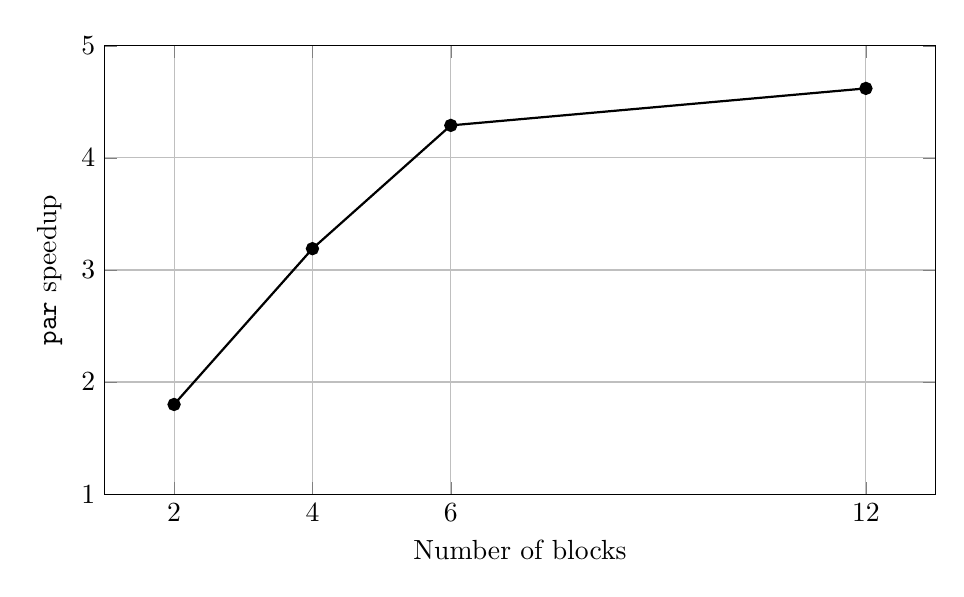
\begin{tikzpicture}
\begin{axis}[
    width=\textwidth,
    height=0.60\textwidth,
    xlabel={Number of blocks},
    ylabel={\texttt{par} speedup},
    xtick={2,4,6,12},
    ymin=1,
    ymax=5,
    grid=major
]
\addplot[
    mark=*,
    thick
] coordinates {
    (2,1.80)
    (4,3.19)
    (6,4.29)
    (12,4.62)
};
\end{axis}
\end{tikzpicture}
\end{minipage}
\end{center}

\noindent
The speedup grows almost linearly up to four blocks, where it reaches $3.2\times$, and then rises more
slowly up to $4.6\times$ with twelve. This means that the parallelism between
blocks is real: adding blocks does not slow down the execution, and the total
time grows much less than the sum of the times. The trend is not linear because the hardware does not scale indefinitely, and because
there remains the part that does not parallelize, that is, the start-up of the interpreter and the
collector, which receives from the channels one at a time.

\section{Limitations}

Three, stated openly. The alphabet of the tests is reduced to three symbols: nothing in the
code depends on it, but nothing exercises it either. The blocks are short, imposed by the
$n^3$ cost of the naive sorting of the rotations, which is the point on which the
reference work itself states that improvements remain necessary. And
the \emph{clean} property in the strict sense, that is,
zeroing the input as well and not only the auxiliary structures, would require the
pair of procedures applied to the whole transform: here the auxiliaries are
zeroed by undoing the procedures that produced them, while the input remains.

% ======================================================================
\chapter{Implementation: interpreter and DAP}
\label{chap:interprete}
% ======================================================================

\section{The chain, from source to execution}

The implementation is split into two halves with a sharp boundary. The first,
written in Python, takes the source down to a textual bytecode; the second, in C,
executes that bytecode in both directions.

\begin{center}
\begin{tabular}{lll}
\hline
& \textbf{stage} & \textbf{output}\\
\hline
\multirow{6}{*}{Python}
 & lexical analysis    & token sequence\\
 & parsing             & syntax tree\\
 & rewriting of \texttt{try} & tree without \texttt{try}\\
 & static checks       & well-formedness errors\\
 & compiled inverses   & \code{p\_\_inv} procedures\\
 & generation          & textual bytecode\\
\hline
C & interpreter        & execution, forward and backward\\
\hline
\end{tabular}
\end{center}

\noindent
The boundary lies in the bytecode, a string of text that the frontend passes
to the interpreter in memory. Using text is a choice made for inspectability: one
can read what the machine executes, and every line carries the line number of the
source it comes from, which is all the debugger needs to stop at the right place.

\section{A step-by-step example}

Consider a procedure that sums the first $n$ integers, with the two-body loop
(\cref{sec:loop}):

\begin{lstlisting}
procedure somma(int n, int s)
    local int i = 0
    from i == 0 do
        s += i
    loop
        i += 1
    until i == n
    delocal int i = n
\end{lstlisting}

\paragraph{Lexical analysis.} The first stage reduces the text to a sequence of
tokens, discarding whitespace and comments. Keywords are not separate regular
expressions: an identifier is recognized and then looked up in a table of reserved
words, so adding a new one costs a single line.

\begin{lstlisting}
PROCEDURE ID(somma) LPAREN INT ID(n) COMMA INT ID(s) RPAREN
LOCAL INT ID(i) EQUALS NUMBER(0)
FROM ID(i) EQEQ NUMBER(0) DO
  ID(s) PLUSEQUALS ID(i)
LOOP
  ID(i) PLUSEQUALS NUMBER(1)
UNTIL ID(i) EQEQ ID(n)
DELOCAL INT ID(i) EQUALS ID(n)
\end{lstlisting}

\paragraph{Parsing.} The grammar is LALR(1), and each production directly
builds the corresponding node. The loop production clearly shows the
relationship between the two:

\begin{lstlisting}
statement : FROM condition opt_do opt_loop UNTIL condition

p[0] = ('from', p[2], p[3], p[6], p.lineno(1), p.lineno(5), p[4])
//               b1    c1    b2                             c2
\end{lstlisting}

\noindent
The two line numbers, that of the \code{from} and that of the \code{until},
allow the debugger to stop at either end of the loop.

\paragraph{Syntax tree.} Nodes are tuples, not objects; statements carry their
line number (conditions do not), and the \code{from} carries two, followed
by the \code{loop} body.

\begin{lstlisting}
('procedure', 'somma', [('int','n'), ('int','s')],
 [('local', 'int', 'i', 0, 2),
  ('from', ('cond','==','i',0),          // entry guard
           [('assign','s','+=','i',4)],  // do body
           ('cond','==','i','n'),        // exit guard
           3, 7,
           [('assign','i','+=',1,6)]),   // loop body
  ('delocal', 'int', 'i', 'n', 8)], 1)
\end{lstlisting}

\noindent
\code{opt\_do} and \code{opt\_loop} are the optional clauses: if they are absent,
the corresponding body is empty.

\paragraph{Bytecode.} Each line consists of a source line number, an opcode, and its
arguments.

\begin{lstlisting}
@1   PROC somma
@1   PARAM int n
@1   PARAM int s
@2   LOCAL int i 0
@3   EVAL i == 0             // entry guard
@3   JMPF FROM_ERR_5
@3   JMP FROM_START_5        // enter, skipping the second body
@3   LABEL FROM_BACK_5
@6   PUSHEQ i 1              //   loop body
@3   LABEL FROM_START_5
@4   PUSHEQ s i              //   do body
@7   EVAL i == n             // exit guard
@7   JMPF FROM_BACK_5        // false: another iteration, going through loop
@7   LABEL FROM_END_5
@7   LABEL FROM_ERR_5
@8   DELOCAL int i n
@1   END_PROC somma
\end{lstlisting}

\noindent
The initial jump realizes the trace $c_1\,[c_2\,c_1]^{*}$: on first entry
the second body is skipped, and control returns to it only via the back-edge. The
labels have structured names (\code{FROM\_START}, \code{FROM\_BACK},
\code{FROM\_END}) because they are also what inversion uses to reconstruct the
loop.

The two assertions of the loop (\cref{sec:loop}), namely $b_1$ true on first entry
(\textsc{LoopError1}) and false on every re-entry (\textsc{LoopError2}), are
needed for inversion: without them the inverse $\mathtt{from}\ b_2\ \mathtt{do}\
\Inv{c_1}\ \mathtt{loop}\ \Inv{c_2}\ \mathtt{until}\ b_1$ could exit after one
iteration while the original performs $n$. This is the same choice made by
Janus~\cite{YokoyamaGluck2007}, and the interpreter checks both: if the entry
guard is false, the jump leads to \code{FROM\_ERR} and execution stops with
\textsc{LoopError1}; when, after the second body, \code{FROM\_START} is reached
again, the interpreter re-evaluates $b_1$ and stops with
\textsc{LoopError2} if it is true. A loop without a $\mathtt{loop}$ clause has
a single body, and the bytecode is shorter: no initial jump and no
\code{FROM\_BACK}, and a false exit guard leads directly back to
\code{FROM\_START}; \textsc{LoopError2} is then checked on that jump.
Likewise, the exit assertion of every
conditional is checked forward after the executed branch and the entry
guard backward, and $\mathtt{local}$ and $\mathtt{delocal}$ form a
block within the same command sequence, as in Janus.

\paragraph{Inversion.} $\mathtt{uncall}$ has two implementations. For a
recursive procedure, even mutually recursive, the frontend applies $\Inv{\cdot}$
to the syntax tree and emits a second procedure, \code{p\_\_inv}, next to
\code{p}: $\mathtt{uncall}\ p$ becomes an ordinary forward call to
\code{p\_\_inv}, with the same loop and the same parameters. For the other
procedures the interpreter inverts the body at run time: it walks through its
bytecode from the last line to the first, using the line index, and executes
for each instruction its inverse (\code{PUSHEQ} becomes \code{MINEQ},
\code{PUSH} becomes \code{POP}, \code{SSEND} becomes \code{SRECV}),
reconstructing loops and conditionals from the labels. This is the default
behavior. With the \texttt{--compiled-uncall} option the frontend emits
\code{p\_\_inv} also for every procedure that contains neither \texttt{par} nor
channels, not even through indirect calls, and \texttt{uncall}~$p$ becomes a
forward call, without reconstructing the inverse at every execution. Procedures
with \texttt{par} or channels remain on the run-time path. The branch of a
conditional is read from the exit assertion and the number of iterations of a
loop from its guards, so here too no history of the data is needed. When,
while inverting a body, the interpreter meets a call to a recursive procedure, it
executes forward its compiled inverse body.

\noindent
For $\mathtt{par}$ the inverse is $\mathtt{par}\ \Inv{c_1}\ \mathtt{and}\
\dots\ \mathtt{and}\ \Inv{c_n}\ \mathtt{rap}$, as in \cref{chap:reversibilita}:
the interpreter relaunches the branches, each executed backward, with
$\mathtt{ssend}$ and $\mathtt{srecv}$ swapped.

\section{Structures and execution loop}
\label{sec:interprete}

\paragraph{Structures.} The store $\sigma$ of the semantics is a \code{Frame}: a
vector of variables, each with a type, a value and, if it is a stack or a channel,
the associated structure. A configuration $\langle \sigma, c\rangle$ is the pair
consisting of the current frame and a pointer to the bytecode line.

The table that translates names into indices is a hash table per frame. It is read
without locks, even by the branches of a \texttt{par}: entries are only added, and
when the table grows a larger copy is built and published with a single atomic
write, so a reader always sees either a complete entry or none.

No structure has a size fixed in advance: neither the recursion depth, nor the
number of branches of a \texttt{par}, nor the parameters of a procedure, nor the
names a frame can contain, nor their length. All of them grow on demand, and the
only limit is the system memory: a branch whose thread cannot be created is a
reported error, not an endless wait.

Every recursive activation works on its own frame, cloned from that of the
procedure with the same name index; the same holds for mutual recursion
and for calls made from a branch of a \texttt{par}. A $\mathtt{local}$
in a nested activation therefore lives in the frame of that activation and does not
touch the outer variable of the same name: this is the per-activation store of the
semantics (\S\ref{sec:scope}). A second $\mathtt{local}$ on the same name in the
\emph{same} activation remains the error that the semantics prescribes.

\paragraph{Main loop.} The bytecode remains text, but at startup
the interpreter scans it once and builds a line index: for
each line, where it begins, where it ends, where its operands begin and its
instruction code. The loop no longer searches for lines nor recognizes the opcode
by comparing strings: it reads the code from the index and selects the instruction
with a \texttt{switch}.

\begin{lstlisting}
opc = g_line_index.op[k];                 /* code from the index */
switch (opc) {
case OPC_PUSHEQ: vm_x_pusheq(vm, fname, fi, d); break;
case OPC_MINEQ:  vm_x_mineq (vm, fname, fi, d); break;
case OPC_XOREQ:  vm_x_xoreq (vm, fname, fi, d); break;
...
\end{lstlisting}

\noindent
A line executed for the first time is parsed from the text. On the second
execution the interpreter decodes it and keeps the result, per thread:
operands already separated and variable and label names already resolved. Expressions
are compiled once into a tree, kept in a cache keyed by content, and are evaluated
from that, not from the text. The labels of each procedure are collected in a first
pass, together with parameters and declarations, and a jump reaches the label's line
through the index, in constant time. The same loop executes the compiled inverse
bodies, which are bytecode like any other; run-time inversion is handled by a second
path of the interpreter that reads the same text backward. None of this changes what
the program computes: the semantics of \cref{chap:semantica} remains the same.

\section{Parallelism}

A \texttt{par} block spawns one system thread per branch. The branches operate on
disjoint portions of the store (\cref{sec:par}), so the store needs no
locks. The only synchronization between branches is the channel, implemented with a mutex and two wait
queues, one for senders and one for receivers: whoever arrives first
enqueues itself, whoever arrives second finds the partner and wakes it, and the exchange
takes place. This is the rendez-vous of \textsc{Par-Comm}.

For the branches to be truly independent, however, they must share nothing even
inside the interpreter: a service structure common to all branches
would make the result depend on the order in which the threads access it. For
this reason every structure that a branch uses is private to the thread, or is read
without locks because it is never modified: the tokenization state is per
thread, and so are the decoded lines, the expression caches
and the pool of freed integer variables; the commands written in the body of a branch use the frame of the procedure
containing the \texttt{par} but each branch has its own stack of open
$\mathtt{local}$s, the check for concurrent writes resides in the individual variable and
not in a global lock, and the name table is consulted without exclusion,
because entries are only added and become visible when they are complete.
A few global locks remain, held for the duration of a short operation and without
the result depending on the order in which threads acquire them: the one that
adds a name or a cloned frame to the tables, the one for the session
state of the channels, the one for the channels to be restored backward
and the one for the output, which keeps the line of each $\mathtt{show}$ intact even when two
branches print at the same moment.

The bytecode is a single one, read by all branches. The program contains only
instructions and no state: everything that changes during execution resides
in the frames. The interpreter never modifies the text or its index, which the branches
share read-only, without locks and without copies. What a branch
derives from a line, that is, its decoding, resides in structures owned by the
thread and is not shared.

\section{The DAP debugger}
\label{sec:dap}

The interpreter exposes a debug interface, and on top of it an extension for
Visual Studio Code\footnote{\url{https://github.com/nicologiuliani6/kairos-vscode-debugger}}
speaks the Debug Adapter Protocol, the protocol through which the editor talks to
any debugger. One sets breakpoints on the Kairos source, steps through the execution
forward and backward one step at a time or up to the next
breakpoint, inspects variables as they change, and
reads the program output in the debug console.

The link between the two sides is what the textual bytecode makes immediate:
every line carries the number of the source line it comes from
(\S\ref{sec:interprete}), so a breakpoint placed on the source
becomes a condition on the executed lines, with no correspondence table
to build and keep aligned. The state shown to the editor is the same store as
the execution, serialized when the editor asks for it: not a copy kept
updated in parallel, but the current frame read at that moment.

\medskip
\noindent
Backward movement is what distinguishes this debugger from an ordinary one,
and it is not an addition to the interface: a step back executes the \emph{inverse}
of the last instruction, that is, the same direction of execution that the language
possesses. The inverse of an operation on data is another operation on data, and
control instructions do not touch the store, so backward they are only
position. A time-travel debugger for an ordinary language must
record and replay; here there is no data to record, because
the information needed to go back is already in the state: the debugger keeps only the
trace of the executed instructions, that is, where to return, not what to restore.
The step back undoes the last instruction that acted on the store or
on the output: control instructions are not stopping points, whereas a
$\mathtt{show}$ is undone by printing again, because it is its own inverse
(\S\ref{sec:show}). A call that has already completed is undone as a whole, with its
inverse, and the same holds for a completed $\mathtt{par}$: the inverse of
$\mathtt{par}\ c_1\ \mathtt{and}\ c_2\ \mathtt{rap}$ is the $\mathtt{par}$ of the
inverses, executed by the threads as on the way forward.

One implementation constraint deserves mention, because it is not accidental: the
step back takes place inside the interpreter loop and not in the layer that
speaks the protocol. The pointer to the current instruction lives in the former, and
modifying the store from the latter would leave it where it was, with position and
memory telling two different stories. Crossing the boundary of a
call is the case that remains out of scope: going up from the beginning of a procedure to the
caller requires reconstructing the activation record, which is not part of
the store but of the machine that executes it. One cannot step back inside a branch of a
running $\mathtt{par}$: an exchange on a channel has an
inverse that requires the partner, and the $\mathtt{par}$ is undone only as a whole.
For the same reason the step back is not available when execution has stopped
inside an $\mathtt{uncall}$ in progress: there an inversion is already being executed,
and it is completed by going forward.

% ======================================================================
\chapter{Related work}
\label{chap:correlati}
\label{sec:related}
% ======================================================================

Three lines of work are close to Kairos: a concurrent extension of Janus,
a reversible concurrent intermediate language, and process calculi with
rollback. We compare them one at a time.

\paragraph{Concurrent Janus.} The work closest in its goals is an
earlier concurrent extension of Janus~\cite{Sammarchi2019}, which adds a
\texttt{fork\,\dots\,and\,\dots\,join} construct and message passing, and
implements them with a compiler to C++ that uses POSIX threads. The starting
problem is the same, and the differences lie in four choices:

\begin{itemize}
  \item \textbf{Definition.} There, the constructs are defined by the C++ code
    into which they are translated; here, by reduction rules. Having a formal
    semantics is what allows us to state and prove reversibility and confluence
    as properties of the language, rather than as the observed behavior of a
    translation.
  \item \textbf{State.} There, threads share a single global state; here, the
    branches operate on disjoint portions of the store. This is a restriction,
    but it is the assumption from which the confluence of interleavings follows
    (\S\ref{sec:par-conf}), which could not be proved with shared memory.
  \item \textbf{Channels.} There, messages pass through queues with a maximum
    capacity; here, through an unbuffered rendez-vous. This is what makes
    $\mathtt{ssend}$ and $\mathtt{srecv}$ exact inverses of each other: on a
    queue they would act on opposite ends, and the inverse of an enqueue would
    not be a receive (\S\ref{sec:chan}).
  \item \textbf{Execution.} There, the program is compiled and runs like any
    other executable, from start to finish: it cannot be stopped halfway, nor
    can it go backward while it is running. Kairos, by contrast, is an
    interpreter, which executes one instruction at a time: the program can be
    stopped at any instruction, its state inspected, and from there execution
    can proceed forward or step back one instruction at a time. This is what
    the debugger offers (\cref{sec:dap}), and it is possible because every
    instruction has an inverse that the interpreter knows how to execute.
\end{itemize}

\paragraph{CRIL.} Among reversible concurrent languages, the closest in
construction is CRIL~\cite{OguchiYuen2024}, which is, however, an \emph{intermediate
language}, not a language in which one writes programs. It extends Mogensen's RIL: a
program is a collection of \emph{basic blocks}, each with a single
three-address instruction and labels for control flow in both
directions, and several block calls can be executed concurrently in
both directions. Its correctness is expressed by \emph{causal safety} and
\emph{causal liveness}.

\begin{table}[H]
\centering
\renewcommand{\arraystretch}{1.25}
\small
\begin{tabular}{l l l}
\hline
 & \textbf{CRIL}~\cite{OguchiYuen2024} & \textbf{Kairos}\\
\hline
Level & intermediate (basic blocks, three-address) & high-level, structured (Janus style)\\
Concurrency & concurrent block calls & explicit \texttt{par\,\dots\,and\,\dots\,rap}\\
Communication & shared variables & synchronous channels, \emph{disjoint} stores\\
Correctness & causal safety / causal liveness & reversibility (\S\ref{sec:rev}), confluence (\S\ref{sec:par-conf})\\
\hline
\end{tabular}
\caption{Kairos and CRIL compared.}
\label{tab:cril}
\end{table}

\noindent
The most important difference is communication: CRIL uses shared variables,
Kairos only channels between disjoint portions of the store, and confluence
follows from this choice. A detailed comparison of the two correctness criteria
remains to be carried out.

\paragraph{Transactions.} For transactions, the point of comparison is the
$\rho\pi$ and croll-$\pi$ calculi~\cite{LaneseMezzinaSchmittStefani2011,%
LaneseLienhardtMezzinaSchmittStefani2013}, where backward execution is
governed by explicit primitives and behaves like a transaction with
compensation. There, a rollback propagates: if a process to be undone has
communicated with another, the other must be undone as well, and handling this
propagation is a large part of the difficulty. Kairos avoids it by forbidding
communication and concurrency inside a $\mathtt{try}\ldots\mathtt{rollback}$
(\S\ref{sec:try}): a transaction remains local to a branch and there is nothing
to propagate. This is a strong restriction, and it is the reason why our transactions
reduce to syntactic sugar; removing it would mean tackling precisely the
problem that those works solve.

% ======================================================================
\chapter{Conclusions and future work}
\label{chap:conclusioni}
\label{sec:concl}
% ======================================================================

We have presented Kairos, a structured imperative language that is both
reversible and concurrent, and we have given its small-step structural
operational semantics, defined as an extension of that of Janus by
Lami, Lanese and Stefani. What Kairos adds to the base are the constructs
needed by a concurrent language and by a language with data: parallel
composition, synchronous communication over channels with inferred protocols, transactions with
compensation, stacks, procedure parameters and local scope. We have defined
the inversion operator, syntactic and computable in linear time, and shown
that backward execution of a parallel block is well defined: the
disjointness of the portions of the store touched by the branches gives the confluence of
the interleavings that do not communicate, and the binary session constraint makes unique
the pairing between a send and the receive that consumes it. That constraint is
guarded as a property of the execution and not of the text, which allows
delegation, that is, the passing of a channel from one holder to another. The language
is realized by an interpreter, on which we have carried out a case study:
the reversible Burrows--Wheeler transform, with the blocks transformed in
parallel, verified on the test vector of the work it starts from, and measured.

\paragraph{Practical maturity.} The sharpest gap is between what the theory says
is possible and what a real compressor would need, and the two algorithms of the
zip standard show it in opposite ways. Dictionary compression holds up:
in the reference reversible version it runs in $\Theta(n)$, like the best
irreversible one, so reversibility costs nothing in complexity. The
transform does not: it costs $O(n^3)$, and the exponent we measure is about $2.8$.
There remains the problem of the naive sorting of rotations, which is the point on which the
reference work itself states that improvements are possible and
necessary: a better sorting is the direction we would indicate first.
As long as it is missing, the blocks remain short, and with short blocks the transform lacks
the material on which to produce the effect for which it exists. Moreover, the
\emph{clean} property in the strict sense is missing: the auxiliary structures are zeroed
by undoing the procedures that produced them, but the input survives
the output, whereas a compressor must consume it.

\paragraph{The language.} The session discipline is partial by construction:
since labelled choice is missing, the type of a channel is determined only when
the two branches of an $\mathtt{if}$ that communicates perform the same actions on
it; where the fragment is not enough, the type remains undetermined. Adding choice would make total what today
recognizes only the provable conflicts. Extending channels to more than two
participants, instead, is not a direct step: with three holders an offer can
have more than one possible partner, forward execution becomes subject to races
and backward execution would no longer know which rendez-vous to undo.
How to preserve a unique pairing in that case is an open question. More
generally, the absence of
races is here an assumption under which the properties hold, not a theorem:
the compiler checks it conservatively and the interpreter reports the
violations it observes, but giving it the form of a type
system, separate from the calculus, is the usual way of guaranteeing it and remains to be done. Asynchronous communication is another natural
extension, with the caveat that it is not a painless addition: it changes what can
be proved about inversion, because a message in transit is a state that the
rendez-vous does not produce.

\paragraph{The implementation.} On the concurrent calculus, the measurement says that
parallelism is achieved, with a speedup of $4.6\times$ at twelve blocks, and
points to what to improve in the part that remains sequential: the collector,
which receives from the channels one at a time. A tree collector, in which the
results are combined pairwise in parallel, would reduce it.

In the interpreter, the program text, with its line index, is a
single one, shared among the branches. The inverse body is produced at compile time for
recursive procedures; for the others the interpreter inverts the bytecode at run
time, unless one asks with \texttt{--compiled-uncall} to
produce it at compile time also for procedures with neither \texttt{par} nor channels. Every
recursive activation, and every procedure called from a branch of $\mathtt{par}$, works on a
frame of its own cloned from that of the procedure; the commands written in the body
of a branch use the frame of the procedure that contains the $\mathtt{par}$, with
a local stack of the branch's own (\S\ref{sec:interprete}).

\paragraph{The missing comparison.} In Kairos, correctness is the property of
reversibility (\S\ref{sec:rev}): if $c$ takes $\sigma$ to $\sigma'$, then
$\Inv{c}$ takes $\sigma'$ exactly back to $\sigma$, and confluence guarantees
that the order in which the branches of a $\mathtt{par}$ alternate does not change the
result. This is a guarantee on the entire execution: $\mathtt{uncall}$ undoes the whole
computation. The literature on concurrent reversible languages, CRIL included,
reasons instead on individual actions and uses two criteria. \emph{Causal safety}
requires that an action can be undone only after undoing all those that
depend on it: a send is not undone if the receiver has already used the value. \emph{Causal
liveness} requires the opposite, that every action whose consequences
have been undone can actually be undone, without getting stuck. The order
of undoing therefore need not be the exact inverse of the forward one:
it suffices that it respect the dependencies.

It is plausible that Kairos also satisfies these two criteria: actions of different
branches do not depend on one another, because they touch disjoint portions of the
store, and the only dependency between branches is the rendez-vous, which with the binary
session is always undone as a pair. \emph{This is not proved, however.} Proving it would
also tell us where this property comes from: if, by allowing branches to share
variables, the two criteria ceased to hold, it would be the choice of having the branches
communicate only through channels that makes them true.

\bigskip
\noindent
Reversibility and concurrency are usually studied separately: the former in
programming languages, the latter in process calculi, with few
occasions for meeting. Kairos is an attempt to have them together in a language
in which programs are written, and the case study is the check that
the combination produces something: a single program that compresses and decompresses,
on blocks transformed in parallel, is something that neither of the two lines of work
achieves alone.
